\documentclass[12pt,a4paper]{book}

\usepackage [english]{babel}
\usepackage [utf8]{inputenc}

%\usepackage[left=2.5cm,right=2.5cm,top=2.5cm,bottom=2.5cm]{geometry}

\usepackage{longtable}
 
%\setcounter{secnumdepth}{3} % le estoy indicando la profundidad hasta donde tiene que mostrar en el indice
%\setcounter{tocdepth}{4} 

\usepackage[titletoc]{appendix}

\RequirePackage[paperwidth=17cm,paperheight=24cm,inner=15mm,outer=20mm,top=25mm,bottom=25mm]{geometry} %%dimensiones externas del pdf y margenes internos.

\usepackage [T1]{fontenc}
\usepackage{graphicx}
\usepackage{graphics}
\graphicspath{ {Figures/} } %Para buscar las imágenes en otra carpeta
\usepackage{amsfonts} %Para poder escribir letras como la matriz identidad
\usepackage{mathrsfs} %Para poder escribir letras como la H del el espacio de Hilbert
\usepackage{slashed} % para la barra cruzada
\usepackage{amsmath}
\usepackage{amssymb}
\usepackage{makeidx}
\usepackage{hepunits} %para poder utilizar unidades
\usepackage[version=3]{mhchem} %para poder escribir los simpolos atómicos y químicos
%\usepackage{hep}

%\renewcommand{\figurename}{ Figura}
%\usepackage[labelsep=endash]{caption}

%\usepackage[figurename=\bold{Figura}]{caption}
%\usepackage [labelformat=empty]{caption}
%\usepackage{wrapfig} %for I can use wrapfigure
\usepackage[font={small, up}]{caption}
\usepackage[caption = false]{subfig} %% for putting several pictures in the same line
\usepackage{hyperref} %hipervinculos del índice
\setlength{\parindent}{4em} %para que interprete la linea en blanco como un \parragraph{}
\setlength{\parskip}{1em}
%\usepackage{subcaption}
%\usepackage[caption = false]{subfig}


\renewcommand{\baselinestretch}{1.15}
%\renewcommand{\thefigure}{}

%para aumentar el espacio entre elementos del índice
\usepackage{setspace}

\bibliographystyle{unsrthep}



\begin{document}
\captionsetup[figure]{labelfont={bf},labelformat={default},labelsep= endash,name={Figura}}
\begin{titlepage}

\begin{center}
%\vspace*{-1 cm}
%\vspace*{1 cm}
%%\begin{figure}[htb]
%%\begin{center}
%%
\includegraphics[scale=0.7]{1Cover_page/Logo1.png}
%%\end{center}
%%\end{figure}
%%\vspace*{0.2 cm}


%\vspace*{0.2in}
{\large Facultad de Física}\\
{\large Departamento de Fisica Atómica, Molecular y Nuclear}\\
\vspace*{0.2in}
\vspace*{0.6in}
\end{center}
\vspace*{-1in}
\begin{center}
\vspace*{1 cm}


\begin{figure}[htb]
\begin{center}

\includegraphics[scale=0.06]{1Cover_page/Logo2.jpg} 
\end{center}
\end{figure}
\vspace*{1 cm}

\begin{large}
%%\textbf{{\large Thesis}}\\
%%\rule{80mm}{0.1mm}\\
%\vspace*{2 cm}

\end{large}
%%\vspace*{0.2 cm}
\begin{Large}
\textbf{\LARGE TRITIUM: Design, construction and commissioning of an in-water tritium detector} \\
\end{Large}
%\vspace*{0.3in}
\vspace*{1.2 cm}

\begin{large}
\textbf{Marcos Martínez Roig}\\
PhD in Physics\\
\today
\end{large}
\end{center}

\vspace*{-1.2 cm}
%\rule{80mm}{0.1mm}\\
%\vspace*{0.1in}
\begin{large}
\begin{flushright}
\item[\bf Under the supervison of:]\quad  \\ 
José Díaz Medina\\
Nadia Yahlali Haddou\\
\end{flushright}
\end{large}

\end{titlepage}


$\ $
\thispagestyle{empty}  %para que no se numere esta pagina
\chapter*{}

\pagenumbering{Roman} %for using romain numbers (page numering)


\begin{flushright}
\textit{Dedicated to \\
my family}
\end{flushright} 

\newpage

\chapter*{Acknowledgements} \label{chap:Acknowledgements}  %pongo el asterisco para que no se numere ni aparezca en el índice
%%\cleardoublepage
\addcontentsline{toc}{chapter}{Acknowledgements} % para que aparezca en el indice de contenidos
AGRADECER A: PEPE, NADIA, MIREIA, ANA, MARQUITOS, ANDREA, COMPAÑEROS DE DESPACHO Y DEL IFIC/UV (NOMBRAR TODOS), GENTE DEL LARAM (TERESA, VANESA, ROSA, CLODO), ANSELMO Y MIGUEL, INGENIEROS DE NEXT, GENTE DE PORTUGAL, Antonio de extremadura, gente de francia... Y PENSAR GENTE QUE ME DEJO POR EL CAMINO. A DAVID CALVO DEL IFIC, A DAVID CANAL DE SAMTEC, A LUIS FERR... DE PETSYS... A LIDON DEL ICMOL... Ana Ros, Jhon Barrio y Gabriela Llosa del IFIMED. Al programa interreg sudoe -> Soporte financiero!

\newpage

\chapter*{Abstract} \label{chap:Abstract}
%%\cleardoublepage
\addcontentsline{toc}{chapter}{Abstract} % para que aparezca en el indice de contenidos
%LEER LOS 2 ABSTRACS DE ANA MAS LOS ABSTRACS QUE TENGO YO DE LAS CONFERENCIAS Y ARTICULOS (ARTICULOS ALEATORIOS MAS EL DE CARLOS, EL MIO, EL DE NADIA, ETC)

%\begin{abstract}
%Texto           del           abstract
%\end{abstract}

\newpage

\chapter*{Nomenclature and Acronyms} \label{chap:NomenclatureAcronyms}  %pongo el asterisco para que no se numere ni aparezca en el índice
%%\cleardoublepage
\addcontentsline{toc}{chapter}{Nomenclature and acronyms} % para que aparezca en el indice de contenidos
\begin{longtable}{p{25mm} c p{120mm} }
\multicolumn{3}{l}{Acronyms:}\\
\\
$OECD$ & --- & Organisation for Economic Co-operation and Development\\
$Btu$ & --- & British termal unit\\
$UN$ & --- & United Nations\\
$UNFCCC$ & --- & United Nations framework convention on Climate change\\
$ITER$ & --- & International Thermonuclear Experimental Reactor\\
$NPP$ & --- & Nuclear Power Plants\\
$DOE$ & --- & Department of Energy\\
$U.S.A.$ & --- & United States of America\\
$U.S.$ & --- & United States\\
$EPA$ & --- & Environmental Protection Agency\\
$LDL$ & --- & Lower Detection Limit\\
$PWR$ & --- & Pressurized Water Reactor\\
$BWR$ & --- & Boiled Water Reactor\\
$PHWR$ & --- & Pressurized Heavy Water Reactor\\
$quasi-real$ & --- & Less than 10 minuts\\
$LSC$ & --- & Liquid Scintillation Counting\\
%$IUPAC$ & --- & International Union of Pure and Applied Chemistry\\
$LWR$ & --- & Liquid Water Reactor\\
$STP$ & --- & Standard temperature ($0\celsius$) and pressure ($1$ atm)\\
$IC$ & --- & Ionization chamber\\
$BIXS$ & --- & Beta Induced X-ray Spectrometry\\
$PMT$ & --- & PhotoMultiplier Tube\\
$SDD$ & --- & Silicon Drift Detector\\
$EEC$ & --- & European Economical Community\\
$SiPM$ & --- & Silicon PhotoMultiplier\\
$ALARA$ & --- & As Low As Reasonably Achievable\\






$T$ & --- & Temperature (ºC).\\
$V$ & --- & Volume (m$^3$).\\


\\
\\
\multicolumn{3}{l}{Atomic and nuclear symbols}\\
\\
$\ce{CO_2}$ & --- & Carbon Dioxide\\
$\ce{CH_4}$ & --- & Methane\\
$\ce{N_2 O}$ & --- & Nitrous oxide\\
$\ce{HFC}$ & --- & Hydrofluorocarbons\\
$\ce{PFC}$ & --- & Perfluorocarbons\\
$\ce{SF_6}$ & --- & Sulfur Hexafluoride\\
$\ce{^{1}_{1}H}$ & --- & Hydrogen\\
$\ce{^{2}_{1}H}$ & --- & Deuterium (Non-radiactive hydrogen isotope, 1 neutron)\\
$\ce{^{3}_{1}H}$ & --- & Tritium (radiactive hydrogen isotope, 2 neutrons)\\
$\ce{^{4}_{2}He}$ & --- & Helium\\
$\ce{^{3}_{2}He}$ & --- & Isotope of the Helium(Non-radiactive, 1 neutrons)\\
$\ce{n}$ & --- & free neutron\\
$\becquerel$ & --- & Becquerel, Nuclear decay number per second\\
$\liter$ & --- & Liter\\
$\becquerel/\liter$ & --- & Becquerel per liter\\
$Ci$ & --- & Curios\\
$Ci/L$ & --- & Curios por litro\\
$yr$ & --- & year\\
$\giga\watt$ & --- & Giga watt\\
$T_{1/2}$ & --- & Half-life time of a radioactive element\\
$\beta$ & --- & Beta decay\\
$\ce{\overline{\nu}_e}$ & --- & Electron antineutrino\\
$\ce{e^-}$ & --- & Electron\\



$\gamma$ & --- & Gamma decay\\
$\alpha$ & --- & Alpha decay\\
\\
\\
\multicolumn{3}{l}{Añadir en un futuro:}\\
\\
D\&D & --- & Decontamination and Decommissioning.\\
DWS & --- & Drinking water standars\\
UDL & --- & Upper Detection Limit\\


NA & --- & Numerical Apertures\\
PMMA & --- & Polymethyl Methacrylates\\
UV & --- & ULtraviolet\\
WLS & --- & Wavelength shifter\\
\end{longtable}


%%añadir bibliografía al indice
\let\OLDthebibliography=\thebibliography
\def\thebibliography#1{\OLDthebibliography{#1}%
\addcontentsline{toc}{chapter}{\bibname}}

%%indice
\tableofcontents

%%lista de figuras
\listoffigures

%\cleardoublepage
\addcontentsline{toc}{chapter}{List of Figures} % para que aparezca en el indice de contenidos

%%lista de tablas
\listoftables

%\cleardoublepage
\addcontentsline{toc}{chapter}{List of Tables} % para que aparezca en el indice de contenidos

%%%%%%%%%%%%%%%%%%%%%%%%%%%%%%% MAIN BODY %%%%%%%%%%%%%%%



\chapter{Introduction}  \label{chap:GeneralIntroduction} %(%(I have to use latin numbers inside of this chapter))
\pagenumbering{arabic} %for using romain numbers (page numering)
%%\setcounter{page}{-1} %%first number of the counter
	\section{Global energy context}
	The energy necessities around the world has been increased a $60\%$ in the last 25 years and they are growing each day due to, mainly, the strong population growth (mundial population has been increased in a $40\%$ between $1990$ and $2015$) and the fast development of emerging countries like China, India and Brazil. \cite{Renovables}. 

On top of that the outlook is that it will keep increasing as you can see in the figure \ref{fig:Wolrd_energy_consumption_a}, specially for countries which don't belong to the OECD like countries which I have said before. In this figure you can see that the energy quantity which will be used on 2040 is expected to be the double of the one which we used in 2000. 

Nowadays, as you can see in the figure \ref{fig:Wolrd_energy_consumption_b}, the most used elements for getting the energy that we use are liquid fuels, coal and natural gas, namely, natural elements. This fact has two problems. On the one hand, natural elements are limitated and this is a problem due to the huge increasing of the energy consumed in the world and, on the other hand, obtaining energy from these natural elements produces large amounts of greenhouses gases (mainlty $CO_2$) which contribute to the environmental contamination, global warming, deforestation, etc. and this is a very big problem, specially right now, since United Nations (UN) did a communication on November 25, 2019 \cite{HighestCO2}, where they claimed that the lifestyle of the world population has not changed in the last years and, as a reason of that, we achieved the highest level of the \ce{CO_2}.

\begin{figure}[]
 \centering
  \subfloat[]{
    \label{fig:Wolrd_energy_consumption_a}
    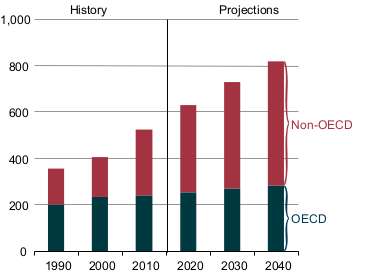
\includegraphics[width=0.5\textwidth]{2Introduction/world_energy_consumption_bar.png}}
  \subfloat[]{
    \label{fig:Wolrd_energy_consumption_b}
    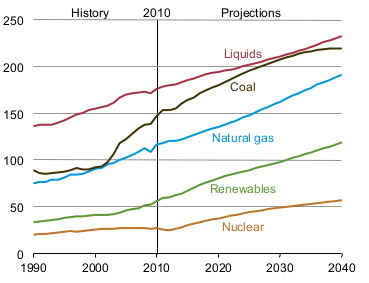
\includegraphics[width=0.5\textwidth]{2Introduction/world_energy_consumption_graph.png}}
 \caption{World energy consumption from 1990 up to now and outlooks for the future until $2040$ (units in $10^{15}~Btu$) \cite{EIA}}
 \label{fig:Wolrd_energy_consumption} 
\end{figure}

In order to control these emissions, the United Nations in the Framework Convention about Climate Change (UNFCCC), has developed a protocol, whose name is Kyoto \cite{Kyoto}. The objective of this protocol is to control and reduce the global negative envirionmental impact. It is focused on 6 different gases, carbon dioxide ($\ce{CO_2}$), methane ($\ce{CH_4}$), nitrous oxide ($\ce{N_2 O}$) and other three types of fluorinate industrial gases ($\ce{HFCs}$, $\ce{PFCs}$ and $\ce{SF6}$), which are related with the greenhouse effect and whose consecuence is the global warming. This convention only encourage to belonging countries to the United Nations to reduce their greenhouses gases emissions but this protocol commits the countries who has signed it to do so.

Therefore, we currently have a problem because, on the one hand, we want to maintain, even increase, this economic growth and for that we need to produce as much energy as we can but, on the other hand, we need to reduce the negative environmental impact. Hence, what we need is a energy source with which we can get a big quantity of energy with a very low greenhouse gases emisions. One possibility which we have is the nuclear fusion plants. They don't emit greenhouse gases and with its energy, which is practically limitless, we could satisfy the humanity's energy necesities .

The largest representative in this sector is the ITER \cite{ITER} (International Thermonuclear Experimental Reactor) that is going to be the largest fusion reactor in the world. The ITER is currently under construction in Cadarache, France, and its objective is to provide the concept of sustained fusion. The reaction which ITER try to reproduce in the earth is the fusion reactor using deuterium ($\ce{^{2}_{1}H}$) and/or tritium ($\ce{^{3}_{1}H}$) because it is the only one whose requirements of temperature (several hundreds of millions degrees) and pressure we can fulfill in the earth. Among the possible combinations between both (table \ref{tab:FusionReactions}), the choice of ITER is the nuclear reaction between deuterium and tritium in a 50:50 mixture because, as you can see in this table,  it is the nuclear reaction with which we get the highest energy release. 

\begin{table}[htbp]
%%\centering
\begin{center}
\begin{tabular}{|c|c|c|}
\hline
Reaction & Products & Energy gain ($\MeV$) \\
\hline \hline \hline
$\ce{^{2}H}+\ce{^{3}H}$ & $\ce{^{4}He}+\ce{n}$ & $17.6$ \\ \hline
$\ce{^{3}H}+\ce{^{3}H}$ & $\ce{^{4}He}+2\ce{n}$ & $11.3$ \\ \hline
$\ce{^{2}H}+\ce{^{2}H}$ & $\ce{^{3}H}+\ce{^{1}H}$ & $3.98$ \\ \hline
$\ce{^{2}H}+\ce{^{2}H}$ & $\ce{^{3}He}+\ce{n}$ & $3.25$ \\ \hline
\end{tabular}
\caption{Fusion reactions between deuterium and tritium\cite{TritiumDocument}}
\label{tab:FusionReactions}
\end{center}
\end{table}

Nevertheles, the fusion power plants is not already prepared for working,  they are still in experimental phase and its researchers need to solve some important problems like inestabilitiy vortex, materials which withstand such high temperatures, etc. \cite{FusionCourse}. Hence, although we know that the future nuclear fusion plants will be the energy of the future, nowadays, we have to wait until all their problems has been resolved.

Other possible  energy source is the existing Nuclear Power Plants (NPPs). With the NPPs we can practically avoid the problem of the greenhouse gases emission. We have to take into account that, although the nuclear fission reaction doesn't emit greenhouse gasses, the total procces to obtain the energy, which involves the uranium mining and milling, transport, uranium enrichment, etc., has a small contribution to the annual release of greenhouses gases. These emissions are difficult to estimate because, on the one hand, they depend on the NPP that we consider (for instance, there are studies which show that asian NPPs has higher emissions \cite{ComparationEmissions}) and, on the other hand, there are some tasks whose greenhouse gases emission are difficult to quantify\cite{ComparationEmissions}. 

There's exist a study \cite{ComparationEmissions} which analyzes $19$ different studies of different NPPs. His estimation for the total greenhouses gases emision of a NPP is $66~\gram~CO_2 /\kilo\watt\hour$ which was obtained as a average of these $19$ studies considered. In the table \ref{tab:ComparationEmisions} this estimation is compared with the estimation for other energy kinds. There you can check that, the emissions due to NPPs is much more smaller, one order or more, than the emissions from burning natural elements.

\begin{table}[htbp]
%%\centering
\begin{center}
\begin{tabular}{|c|c|}
\hline
Technology & Estimate ($\gram~CO_2 /\kilo\watt\hour$)\\
\hline \hline
Wind & $9-10$ \\ \hline
Hydroelectric & $10-13$ \\ \hline
Biogas & $11$ \\ \hline
Solar thermal & $13$ \\ \hline
Biomass & $14-41$ \\ \hline
Solar PV & $32$ \\ \hline
Geothermal & $38$ \\ \hline
Nuclear & $66$ \\ \hline
Natural gas & $443$ \\ \hline
Fuel cell & $664$ \\ \hline
Diesel & $778$ \\ \hline
Heavy oil & $778$ \\ \hline
Coal & $960-1050$ \\ \hline
\end{tabular}
\caption{Estimations of $\ce{CO_2}$ emissions for several kinds of energy sources\cite{ComparationEmissions}}
\label{tab:ComparationEmisions}
\end{center}
\end{table}

NPPs are already working and, nowadays, they are essential for providing a big part of the electic power that is used in the current world (more than a 20\% in Spain as you can see in the table \ref{tab:PercentageEnergySpain}). 

\begin{table}[htbp]
%%\centering
\begin{center}
\begin{tabular}{|c|c|c|c|}
\hline
Type of energy source & Contr. & Type of energy source & Contr.  \\
\hline \hline
Nuclear & $22.0\%$ & Wind & $20.9\%$  \\ \hline
Coal & $4.2\%$ & Hydraulics & $9.7\%$  \\ \hline
Combined Cycle & $20.1\%$ & Solar Photovoltaic & $3.5\%$  \\ \hline
Cogeneration & $11.8\%$ & Solar thermal & $2.0\%$  \\ \hline
No-renewable waste & $0.8\%$ & Other renewables & $1.4\%$  \\ \hline
Pumping turbine & $0.6\%$ & renewable waste & $0.3\%$  \\ \hline
 &  & \parbox{11em}{\centering Impoted balance of\\  international exchanges} & $2.7\%$\\ \hline
\end{tabular}
\caption{Contribution of each energy source to the total energy consumed in Spain in 2019 \cite{PercentageEnergySpain}}
\label{tab:PercentageEnergySpain}
\end{center}
\end{table}

NPP is one of the cheapest source. It is a stable source which doesn't depend on  meteorological parameters and, although there are other alternative energy sources which are being developed quickly  (photovoltaic, wind, tidal energy, etc.), even other concepts of energy production and saving (local production, solar roofs, energy efficiency, smart cities, etc.), today they are not develop enough.  

The detractors of nuclear energy argue that NPPs facilitate nuclear proliferation or there are a risk of radiactive contamination and accidents like it happened in the past: Chernobyl, Fukushima and other accidents with lesser impact such as Three Mile Island, near to Pensilvania, USA.

Although we know that the nuclear energy is not the energy of the future since it produces nuclear waste which, by the moment, we don't know how we can eliminate, it is difficult that we leave to use nuclear energy because, now, we don't have a better solution for obtaining the energy which we need. 

In Spain the government are doing an effort in order to remove all nuclear power plants. This is because they are not going to build new nuclear reactors and they are only waiting until the NPPs have reached the end of their useful life (approximately 40 years). They expect to close all NPPs between $2020$ and $2030$ \cite{CloseNPP}. 

Other countries like France, where the $77\%$ of their energy consumed is obtained from nuclear sources, prefer to maintain their nuclear facilities and there's even exist other countries that believe that nuclear energy is a safe investment like China who announced in 2016 that they were going to build 60 new nuclear reactors in the next dedade \cite{60ReactorsChina} or USA, who made an investment of 35 million of euros in 2019 for development and improvement of nuclear power plants \cite{35MillionsUSA}. 

In any case it is not important if we agree or not with nuclear energy source. The only important thing is that the nuclear energy production in the world is not going to stop in the next decade, in fact, it will increase as you have seen in the outlooks of the figure \ref{fig:Wolrd_energy_consumption_b}. Therefore the development of  different types of alarm systems is a good investment of both, time and money. Safety is not a negotiable aspect and there must be mechanisms that warn us of any malfunction of a nuclear power plant. Hence, our work has based on the development of a monitor that we can use as early alarm in case of any problem happen in a NPP.

Generally, a nuclear reactor, which is working in normal mode, is characterized by extreme stability and, therefore, by a constant emission of radioactive isotopes so the first alarm signs of any malfunctioning of a NPP is a variation of this radiactive emission rate.

Between all the radioactive elements which is produced in a nuclear power plant, the most frequently produced is tritium as DOE complex \cite{FiberDetector1a} \cite{FiberDetector1b}  and other research facilities in China \cite{CommonEmissionTritium} have seen in their installations and in ground water, surface water, and process waste water around their facilities. However, as we will see in the section \ref{sec:StateOfTheArt}, the current methods which is used for monitoring this radioactive element has some limitations. 

Therefore, the radiactive element which we have chosen for monitoring with our early alarm system is tritium. We have focused our alarm system for working with NPPs but it could be also interesting for other tasks where tritium is involved like monitoring the behaviour of future fusion nuclear plants (ITER will need up to several tens of kilograms of tritium for working, which correspond to several $\tera\becquerel$ of tritium.) or any nuclear research facility (tritium is a commun emission of these places \cite{FERMILAB},\cite{BrookHavenNationalLaboratory}),  tracking the movement of tritium contaminated plumes in ground water \cite{TrackingTritium} or demonstrate the compliance with the government agencies which fix the limit of the emitted radionuclides to the environmental. 

We have to take into account that the limit of the emission of each radioactive element depends on the government agency who manages it, and the regulation directives that is implemented in that place so, as a consequence, it is different in each country. For example, in Europe, the agency is Council Directive and the limit which they have stablished for tritium in drinking water is $A = 100~\becquerel/\liter$ \cite{100BqL}. In USA, the organization is United States Envirnomental Protection Agency (U. S. EPA) and this limit is $A = 20~\nano\curie/\liter = 740~\becquerel/\liter$ \cite{740BqL}.

Tritium is normally produced in the water that there are in the cooling system or the moderator of some NPPs. It usually appear by neutron capture of the deuterium, which exist in the heavy water ($D_2 O$), semi-heavy water ($H D O$) or the deuterium which has created by neutron capture in usual water ($H_2 O$). All these processes have a big probability to happen due to the huge quantity of neutrons which we has in the nuclear reactor, $10^{14} ~\ce{n} \, \cm^{-2} \second^{-1}$ \cite{CrossSeccionNeutrons}. 

The quantity of tritium will be different for each reactor type because, as we will see in the next seccion, the cross section of tritium production will depend on the materials which there are in any type of NPP. In the table \ref{tab:TritiumEmisionsNPPs} we can see the emissions of different types of nuclear reactors:

\begin{table}[htbp]
%%\centering
\begin{center}
\begin{tabular}{|c|c|c|}
\hline
Reactor type & Gaseous discharge ($\giga\becquerel/$y) & Liquid discharge ($\giga\becquerel/$y) \\
\hline \hline \hline
PWR & $3.70\cdot 10^{3}$ & $2.59\cdot 10^{4}$ \\ \hline
BWR & $1.85\cdot 10^{3}$ & $3.70\cdot 10^{3}$ \\ \hline
HWR & $7.40\cdot 10^{5}$ & $1.85\cdot 10^{5}$ \\ \hline
GCR & $7.40\cdot 10^{3}$ & $1.11\cdot 10^{4}$ \\ \hline
\end{tabular}
\caption{Emission of tritium in several different types of nuclear reactors\cite{CommonEmissionTritium}}
\label{tab:TritiumEmisionsNPPs}
\end{center}
\end{table} 

The tritium which is created in the water of the cooling system is finally released partially or totally to the environment. Between these types, the most common way is $\ce{HTO}$ \cite{CommonEmissionTritium}.

Our alarm system will monitor the activity of tritium in the water of the cooling system of the NPP which is emitted to the environmental. It can also work for the water of the moderator in these types of NPP but it's not our objective because it's a close circuit so it's not a emission (unless the moderator is leaking, in which case our alarm system would detect it indirectly due to a variation of tritium activity in the water of the cooling system released to the environment).

The measurement of the tritium activity is one of the systematic environmental control which is performed during energy production by NPPs. It is normally done by LSC technic which has a very good detection capability and precision but it has some problems, for example, it needs too long time for taking a measurement (2 days or more). I will speak more about LSC technic in the section \ref{sec:StateOfTheArt}.

The detection of this tritium in quasi-real time ($<10~\min$) is important because of the following reasons:

\begin{enumerate}

\item{} It can warn us about the production of an excesive number of neutrons in the nuclear reactor due to the overheating of itself or a leakage of the water from the primary circuit of the cooling system in a nuclear power plant due to some break (perhaps because of an excesive preassure, other alarm sign of a malfunctioning of a nuclear reactor). Both causes could become in a very dangerous problems so the tritium detection in quasi-real time could be important in order to quickly detect and to solve it.

\item{} This water, which there are in the secondary circuit of the cooling system, will be released to the eviromental, usually rivers or seas, after using it for cooling purposes. Generally this water will be used for human consuming, irrigation of all kind of plantations or it will arrive to a places where we fish. 

Due to such a low legal limit in comparation with the activities of tritium inside of a nuclear reactor, it is possible that, if the nuclear power plant don't work correctly, the activity of tritium water released will overcome this limit and it become this water in no drinkable and these crops into inedibles. On top of that, the life time of tritium is more than 12 years so these places will remain contaminated during a lot of time. 

\item{} There's exist a lot of rivers or seas, which is used for cooling systems of the nuclear power plants, that are crossborders, that's, they are shared by several countries like our case as we will see in the seccion \ref{sec:TritiumProject}. The emisión of an excessive tritium activity of one country could be affect severely to the other country creating new international conflicts between them.

\end{enumerate}

Because of all these reasons it is very important that we have an alarm system which is capable of measuring such low tritium activities in quasi-real time. Nevertheless, as we will see in the section \ref{sec:StateOfTheArt}, currently there are not any technic with which we can fulfill these requeriments.

All these reasons has motivated the project \textit{Tritium}, whose objective is the development of a system for quasi-real time monitoring of low radioactive levels of tritium in water for security applications in nuclear power plants. \label{sec:Introduction}
	\newpage

	\section{Tritium properties}
	Tritium is the only radioactive isotope of hydrogen. It was first time produced in $1934$ from neutron capture of deuterium by Ernest Rutherford, Mark Oliphant and Paul Harteck \cite{TritiumDiscovery} and it was first time isolated in 1939 by Luis Walter Alvarez and Robert Cornog \cite{TritiumIsolate}, who checked that tritium is a radiactive element. 

Tritium can be found in the environment since it is normally produced through the interaction of cosmics rays and gaseous elements of the upper atmosphere like nitrogen ($\ce{^{14}N}(\ce{n},\ce{^{3}H})\ce{^{12}C}$) \cite{TritiumHandling} and oxigen ($\ce{^{16}O}(\ce{n},\ce{^{3}H})\ce{^{14}N}$) \cite{OxigenTritium}. Then tritium becomes water (\ce{HTO}) and reaches the earth's surface as rain with an estimated produccion rate of $4\cdot 10^6 ~\curie/$yr \newline ($1.48 \cdot 10^8 ~\giga\becquerel/$yr) \cite{CommonEmissionTritium} \cite{TritiumHandling} . 

Tritium can be produced artificially in the environment from many different anthropogenic origins. There are a big amount of tritium which was produced on militar nuclear test explosions between 1945 and 1975, whose estimed produccion rate is $8 \cdot 10^9~\curie$ ($2.96 \cdot 10^11~\giga\becquerel$) and a part of that still remain. It was mainly produced from the nuclear reactions $\ce{^{14}N}(\ce{n},\ce{^{3}H})\ce{^{12}C}$ and $\ce{^{2}H}(\ce{n},\gamma)\ce{^{3}H}$. Tritium can be also produced by commercial producers of radioluminicent and neutron generator devices ($1 \cdot 10^6$ $~\curie/$yr), nuclear power and defense industries (less than $2 \cdot 10^6~\curie/$yr), several research facilities and nuclear reactor operation ($2 \cdot 10^6 \curie/\giga\watt$yr), whose main production channels are \cite{CommonEmissionTritium} \cite{TritiumHandling}:

\begin{equation}
\ce{^{2}_{1}H}(\ce{n},\gamma)\ce{^{3}_{1}H} \qquad \sigma_{th}= 5.2 \cdot{} 10^{-4}~\barn  ~~~\cite{CommonEmissionTritium}
\label{capneuH2}
\end{equation}

\begin{equation}
\ce{^{3}_{2}He}(\ce{n},\ce{p})\ce{^{3}_{1}H} \qquad \sigma_{th}= 5330~\barn ~~~\cite{CommonEmissionTritium}
\label{capneuHe3}
\end{equation}

\begin{equation}
\ce{^{6}_{3}Li}(\ce{n},\alpha)\ce{^{3}_{1}H} \qquad \sigma_{th}= 940~\barn ~~~\cite{CommonEmissionTritium}
\label{capneuLi6}
\end{equation}

%%\begin{equation}
%%\ce{^{7}_{3}Li}(\ce{n},\alpha)\ce{^{3}_{1}He} + \ce{n} ~~~\cite{CommonEmissionTritium}
%%\label{capneuLi7}
%%\end{equation}

\begin{equation}
\ce{^{10}_{5}B}(\ce{n},2\alpha)\ce{^{3}_{1}H} \qquad \sigma_{th}= 3835~\barn ~~~\cite{CommonEmissionTritium}
\label{capneuB10}
\end{equation}

%\begin{equation}
%\ce{^{11}_{5}B}(\ce{n},2\alpha)\ce{^{3}_{1}H} + n ~~~\cite{CommonEmissionTritium}
%\label{capneuB11}
%\end{equation}
%$\eqref{capneuLi6}$ para referenciar ecuaciones

%There are two more nuclear reaction with which we can produce tritium:

%\begin{equation}
%\ce{^{1}_1 H} (2 \cdot{} \ce{n},\ce{p})\ce{^{3}_1 H}
%\label{doblecapneuH}
%\end{equation}

%\begin{equation}
%\ce{^{2}_1 H}(\ce{n},\gamma)\ce{^{3}_1 H}
%\label{capneuD}
%\end{equation}

Tritium is a radioactive element whose half-life time is $T_{1/2}= 12.32$ years. It has one proton and two neutrons and decays exclusively through $\beta$ radiation, that's, it doesn't have other type of radioactive decay. In this decay, one neutron of tritium is transformed in a proton plus electron and electron-antineutrino according to the following equation:

\begin{equation}
\ce{n} \longrightarrow \ce{p^+}  + \ce{e^-}  + \ce{\overline{\nu}_e}
\label{BetaDecay}
\end{equation}

Then the nucleus of the tritium son has two protons and one neutron so it is a helium isotope, $\ce{^{3}_{2}He}$ which is stable. Therefore, the nuclear reaction which descript the $\beta^-$ decay of the tritium is:

\begin{equation}
\ce{^{3}_{1}H} \longrightarrow \ce{^{3}_{2}He}  + \ce{e^-}  + \ce{\overline{\nu}_e}
\label{TritiumDecay}
\end{equation}

In the Figure \ref{fig:TritiumDecay} we can see the scheme of tritium energy levels. In this decay we practically don't have the posssibility of detecting the neutrinos because it interacts very weakly with matter and, therefore, with our detector ($\sigma \propto 10^{-42} ~ \cm^2$ \cite{CrossSeccionNeutrino}) and, since $\ce{^{3}He}$ has a much larger mass than electrons and neutrinos, by conservation of energy and momentum, the energy that is taken by its atom is very small. Therefore, we will focus on the electron detection. 

\begin{figure}[hbtp]
 \centering
  \subfloat[Tritium energy levels \cite{TritiumDecayEnergyLevels}]{
   \label{fig:Energy_levels}
    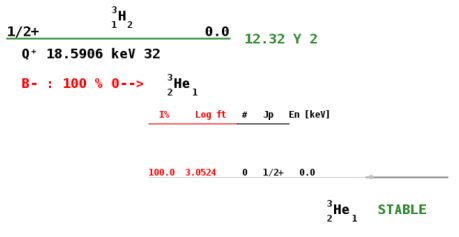
\includegraphics[width=0.47\textwidth]{2Introduction/esquema_niveles_energeticos.png}}
  \subfloat[Graphic representation of tritium decay \cite{TritiumDecayImage}]{
   \label{fig:GraphicDesintegration}
    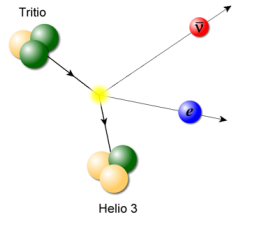
\includegraphics[width=0.53\textwidth]{2Introduction/representacion_desintegracion.png}}
 \caption{Tritium decay}
 \label{fig:TritiumDecay}
\end{figure}

The energy that is released in this nuclear reaccion is constant, $18.6~\keV$, but it is divided between the products of this reaccion. Therefore not all beta particle (electrons) will have the maximum energy. This is what we can see in the figure \ref{fig:TritiumDecaySpectrum}, which is the energetic spectrum of the electrons which are emitted in the tritium decay. The maximum energy of this electrons is $18.6~\keV$ (when beta particles have all the energy), which is the endpoint energy of this spectrum, the average energy is $5.7~\keV$ and the most likely value is slightly below of the average energy, around $4.5~\keV$.

\begin{figure}[hbtp]
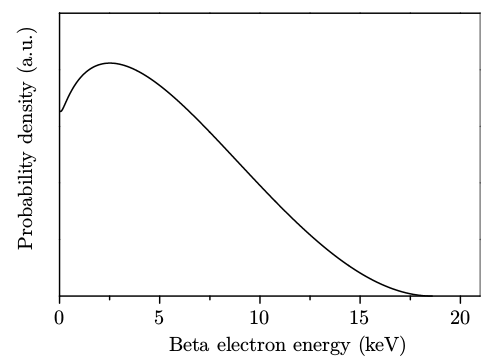
\includegraphics[scale=0.6]{2Introduction/Espectro.png}
\centering
\caption{Energy spectrum of tritium electrons ~\cite{TesisTritio}\label{fig:TritiumDecaySpectrum}}
\end{figure}

Keep in mind that, although the helium isotope is stable, it will be exited immediately after this decay. As a consequence, after the tritium $\beta^-$ decay, we will have a subsequent dexcitation of the $\ce{^{3}He}$ which will produce fotons, $\gamma$, with several well-defined energies that correspond to their energy levels, X-rays. COMPROBAR... It doesn't affect directly to our detector due to the efficiency of our detector at those wavelenghts, as we will se in the chapter \ref{}, section \ref{},  but it could be affect indirectly. BUSCAR ESTAS ENERGÍAS Y VER SI SON TAN DIFERENTES COMO PARA NO AFECTAR DIRECTAMENTE O SE PARENCE A LAS DEL TRITIO Y SI AFECTAN DIRECTAMENTE.

The releasing energy, which is produced in the tritium decay, is very little. In fact, it is the radioactive isotope with the lowest energy released in its $\beta$ disintegration \cite{TritiumHandling}. As a consequence the $\beta$ particles which is emitted in this tritium decay will have a very little mean free path as you can see in the table \ref{MeanFreePathTritium}.

\begin{table}[htbp]
\begin{center}
\begin{tabular}{|c|c|c|}
\hline
Material & Energy ($\beta$)(keV) & Penetration Depth \\
\hline \hline \hline
$\ce{\ce{^{3}_{1}H_2}}$, STP & 5.7 & 0.26 cm \\ \hline
$\ce{\ce{^{3}_{1}H_2}}$, STP & 18.6 & 3.2 cm \\ \hline
Air, STP & 5.7 & 0.036 cm \\ \hline
Air, STP & 18.6 & 0.45 cm \\ \hline
\parbox{10em}{\centering Water, soft tissue\\  (solid matter whose \\  density is $1~\gram\cdot\cm^{-3}$)} & 5.7 & 0.42 $\mu\meter$\\ \hline
\parbox{10em}{\centering Water, soft tissue\\  (solid matter whose \\  density is $1~\gram\cdot\cm^{-3}$)} & 18.6 & 5.2 $\mu\meter$ \\ \hline
\end{tabular}
\caption{Mean Free Path of tritium isotope for several energies~\cite{TritiumHandling}}
\label{MeanFreePathTritium}
\end{center}
\end{table}

On the one hand, it means that the tritium electrons is easily stopped even for simply walls like our clothes, the laboratories gloves or even the our skin it-self, that's, the radioactive hazard is low. Nevertheless, the danger of tritium is increased when tritium is ingested or inhaled because if it has enough radiactivity it can affect to our internal organs because it has a high biologic life time, $9.5$ days \cite{TritiumHandling}, time during which tritium remains in our body and we will be receiving dose due to tritium radiation. Therefore, their health hazard is high.

On the other hand, this short mean free path will be a problem when we try to detect tritium and due to that, there are some limitations which we will have to take into account when we design our detector. 

Tritium has different physical properties than other natural isotopes of the hydrogen like different boilling points as you can see in the table \ref{BoillingPoints} or the property of auto-radiolysis which only happens when radioactive elements are presented. The auto-radiolysis exists because the energy released in tritium decay is larger than the energy bond of oxigen and hydrogen in water molecules ($5.2~\eV$) or the ionization energy of water molecules ($12.6~\eV$) so it can break up these molecules \cite{AutoRadyolisis}. Due to the auto-radiolysis, some radicals appear in the water whose corrosivity is increased.

\begin{table}[htbp]
\begin{center}
\begin{tabular}{|l|l|l|}
\hline
Molecule & Boiling point (for gases) ($\kelvin$) & oxidation form\\
\hline \hline \hline
$\ce{H_2}$ & 20.39 & $\ce{H_2 O}$ \\ \hline
$\ce{HD}$ & 22.14 & $\ce{HDO}$ \\ \hline
$\ce{HT}$ & 22.92 & $\ce{HTO}$ \\ \hline
$\ce{D_2}$ & 23.66 & $\ce{D_2 O}$ \\ \hline
$\ce{DT}$ & 24.38 & $\ce{DTO}$ \\ \hline
$\ce{T_2}$ & 25.04 & $\ce{T_2 O}$ \\ \hline
\end{tabular}
\caption{Gas molecules of hydrogen isotopes and their boiling points}
\label{BoillingPoints}
\end{center}
\end{table}

Although tritium has different physical properties it has almost the same chemical behaviour than other hydrogen isotopes. Tritium, like hydrogen, is a gas at standard conditions of temperature ($273~\kelvin$) and preassure ($1$ atm) forming a two-atom molecules which can be $\ce{HT}$, $\ce{DT}$ and $\ce{T_2}$. It can become in tritium water through oxidation and exchange reactions as you can see in the following chemical ecuations\cite{TritiumHandling}:

\begin{equation}
\begin{split}
& Oxidation: \qquad \qquad \qquad \qquad \qquad \qquad Excahnge\\
& 2\cdot{}\ce{HT} + \ce{O_2} \rightarrow 2 \cdot{} \ce{HTO} ~ \quad \qquad \qquad \qquad \ce{HT} + \ce{H_2 O} \rightarrow \ce{H_2} + \ce{HTO}\\
& 2\cdot{}\ce{T_2} + \ce{O_2} \rightarrow 2 \cdot{} \ce{T_2 O} \qquad \qquad \qquad \qquad \ce{T_2} + \ce{H_2 O} \rightarrow \ce{HT} + \ce{HTO}
\label{OxidationExchange}
\end{split}
\end{equation}

Due to this chemical similarity tritium water can performe the same chemical process than non-radiactive water, some times with higher rate if the tritium concentration is high enough to catalyze the reaction. Its biological hazard comes from this chemical similarity since tritium water is able to substitute normal water in human body. On top of that, tritium water has a higher absorption in human body, around 99\%, than tritium gas, whose absorption in the human body is less than $5 \cdot 10^{-3}\%$  by inalation or practically negligible by skin absorption \cite{TritiumHandling} so it is more dangerous.\label{sec:TritiumProperties}
	\newpage
	
	\section{State-of-the-art in tritium detection}
	Measurement of tritium activity is one of the systematic environmental controls that have been carried out for dozens of years around nuclear power plants during their energy production and around nuclear research facilities.

As a consequence, this measurement has been attempted with many different technologies so far in order to improve the state of the art of each time. The most researched techniques are summarized in the table \ref{DifferentThecnics}.

\begin{table}[htbp]
\begin{center}
\begin{tabular}{|c|c|c|c|c|}
\hline
 & LSC & IC & Calorimetry & BIXS\\
\hline \hline \hline
\parbox{5em}{\centering Measured\\ quantity} & \parbox{5em}{\centering Scintillation\\ photons} &  \parbox{5em}{\centering Ionization\\ current} & heat & X-rays\\ \hline
LDL & $\sim\becquerel$ & $10-100~\kilo\becquerel$ & $\sim~\giga\becquerel$ & $\sim~\mega\becquerel$ \\ \hline
Sample form & Liquid & Gas, vapor & All & All \\ \hline
%Disadvantages & & Gas, vapor & All & All \\ \hline
\end{tabular}
\caption{State-of-the-art in the tritium detection for different technics~\cite{TesisTritio}}
\label{DifferentThecnics}
\end{center}
\end{table}

Nowadays, the most used technic for mesuring tritium in water is the LSC. It consists of mixing a liquid sample (some ml for environmental measurements or less for higher activities) with liquid scintillator. In our laboratories, LARAM, at the University of Valencia, this mixture is made in a ratio of 50:50 \cite{LSCLARAM} but it will depend on each system and each sample \cite{LSCothers} \cite{HofstetterSeveral}. In this technic, the $\beta$ energy that is emitted from the sample excites the molecular energy levels of the liquid scintillator and it is quickly desexcited emitting several photons with a well-know energy (fluorescence), normally in the visible range. Finally these photons are detected with photosensors, processed and analysed.

This technic has a very good detection capability and precision (LDL for tritium better than $1~\becquerel/\liter$ \cite{0.6Bq_L}) but it has some problems. On the one hand it need too time for taking a mesurment (more than $2$ days) and, on the other hand, although this sample could be non-radiactive, it contain tolueno which is a toxical chemical waste so we need to follow a special protocol for removing this samplex. On top of that all these technics need special staff for sampling, chain-of-custody and lab analysis which consum economical and time resources. In order to avoid the last problem a monitor of tritium with LSC has been studied \cite{OnlineLSC} but the other problems still remain. 

The ionization chamber (IC) is based on a gas chamber (sample) which contains electrodes connected to different voltage. This electrodes recover the ionization current that is produced due to the $\beta$ radiation. It is a simple and fast system, but the problem is that on the one hand it has too high LDL, more than $ 10~\kilo\becquerel$, and, on the other hand, it needs the state of the sample to be gas or steam \cite{IonizationChamber1} \cite{IonizationChamber2}.

The calorimetry is based on the measurement of the heat generated due to the tritium radiation \cite{Calorimeter1} \cite{Calorimeter2}. The problem with this technic is that it has a too high LDL, of the order of $\giga\becquerel$, and it needs too long time, more than 2 days, for taking a measurement.

The Beta Induced X-ray Spectrometry (BIXS) is based on the measurement of the bremsstrahlung with PMTs of \ce{NaI} \cite{XRays1} \cite{XRays2} or with Silicon Drift Detector (SDD) \cite{Bremstrahlung} produced due to the tritium radiation. The problem with this technic is that it has too high LDL, of the order of $\mega\becquerel$.

There are many more different methods for tritium detection, although they are less used or less experimentally developed, each one with their own problems for our objective. For example,  APD \cite{APD}, which we cannot use in our case because they cannot function in contact with water, the mass spectrometry \cite{Spectrometry}, which needs to store the sample several months before taking the measurement or Cavity ring spectroscopy \cite{Ring}, which requires a special optical configuration that is not possible outside the laboratory.

We have to keep in mind that all these techniques are offline methods that take too long to finish the process of taking measurements which include sample taking, sending the sample to the lab, analyzing of the sample so we cannot use them for tritium monitoring. LSC is the only technic which has a LDL enough low to verify the compliance with the established limit, $100~\becquerel/\liter$. Therefore we will explore this area but, in order to avoid the problems related with this technic (off-line results, no-reusable liquid scintillator and the chemical toxic wastes) we will delve in solid scintillators. There are several studies that have been done so far which intend to do the same as we want with this project, to create a quasi-real time monitor of low tritium activities in water based on solid scintillation:

\begin{itemize}

\item{} First study was done by M. Muramatsu, A. Koyano and N. Tokunaga in 1967 who used a scintillator plate read out by two PMTs in coincidence \cite{Muramatsu}.

\item{} The second study was carried out by the A. A. Moghissi, H. L. Kelley, C. R. Phillips and J. E. Regnier in 1969 that used one hundred plastic fibers coated with anthracene powder and read out by two PMTs in coincidence \cite{Moghissi}.

\item{} Third study was performed by R. V. Osborne in 1969 who used sixty scintillator plates stacked read out by two PMTs in coincidences \cite{Osborne}.

\item{} Fourth study was done by the A. N. Singh, M. Ratnakaran and K. G. Vohra in 1985, who used a scintillator sponge read out by electronic coincidence \cite{Ratnakaran}\cite{Ratnakaran2000}.

\item{} Fifth study was carried out by K. J. Hofstetter and H. T. Wilson in 1991, who did different experiments for testing different shapes of scintillator plastic like several sizes of beads, fibers, etc. The better result which Hofstetter got for solid plastic scintillator was a efficiency of the order of $10^{-3}$ \cite{Hofstetter1}\cite{Hofstetter2}.

\end{itemize}

\begin{table}[htbp]
\begin{center}
\begin{tabular}{|c|c|c|c|c|}
\hline
 & \parbox{6em}{\centering Efficiency, $\eta_{det}$\\ $(cps/(\kilo\becquerel/\liter))$}  & \parbox{5em}{\centering Surface\\ $F_{sci}$ ($\cm^2$)}  & \parbox{5em}{\centering Specific efficiency\\ $\varepsilon_{det}=\eta_{det}/F_{sci}$} & LDL ($\kilo\becquerel/\liter$)\\
\hline \hline \hline
Muramatsu & $3.85 \cdot 10^{-4}$ & $123$ & $3.13 \cdot 10^{-6}$ & $370$ \\ \hline
Moghissi & $4.5 \cdot 10^{-3}$ & $>424.1$ & $<1.06 \cdot 10^{-5}$ & $37$ \\ \hline
Osborne & $0.012$ & $3000$ & $4 \cdot 10^{-6}$ & $37$ \\ \hline
Singh & $0.041$ & $3000$ & $1.37 \cdot 10^{-5}$ & $<37$ \\ \hline
Hofstetter & $2.22 \cdot 10^{-3}$ & $\sim~100$ & $<2.22 \cdot 10^{-5}$ & $25$ \\ \hline
\end{tabular}
\caption{Results of different scintillator detector for tritium detection~\cite{TesisTritio}}
\label{PlasticScinTritium}
\end{center}
\end{table}

%COMPROBAR QUE ESTAN BIEN TODOS LOS DATOS (sobretodo areas, lo otro esta comprobado. A lo mejor puedo calcular el area del ultimo caso)

The results of these experiments are sumarized in the table \ref{PlasticScinTritium}. We can see in the first column that the intrinsic detector efficiency, $\eta_{det}$, is very different in these experiences. As we know that, in this type of detectors, one of the most important factor, which affect to the efficiency, is the active surface of the plastic scintillator, $F_{sci}$, and we can see in the second column that it is very different en each detector, we use the specific detector efficiency (third column), in order to compare these experiments, that's, the efficiency normalized to this active surface. Now we can check that, effectively, these specific efficiencies are quite similar. On top of that we can check that the better specific efficiency was obtained for Moghissi who used scintillating fibers. This is a good point which justify our choice about using of fibers like a scintillator. Finally we can see in the last column that the LDL in all these experience are more or less similar and, they are too high for our aim. 

To sum up with solid scintillator detectors we can practically avoid all the different problems which other techniques have. The only problem which still remain is that they have a too high LDL. Developing a detector which overcome these LDL is an essential study right now in order to monitoring the tritium levels.\label{sec:StateOfTheArt}
	\newpage
	
	\section{Tritium project and Tritium monitor}
	As we have seen in the section \ref{sec:StateOfTheArt}, the current technics which exist nowadays have either higher LDL than the limit established by Council Directive, $100~\becquerel/\liter$, or they are a off-line method (too slow) so those methods cannot be used for tritium monitoring in quasi-real time. 

As a result of these limitations appear the \textit{Tritium} project \cite{TRITIUM}, whose title is "Design, construction and commissioning of automatic stations for quasi-real time monitoring of low radioactive levels of tritium in water".

This project has been funded by Interreg Sudoe program of the EEC in the 2016 call with the reference number SOE1/P4/EO214. The purpose of this project is the development of a tritium monitor in quasi-real time. This monitor consists of a ultra pure water system, which prepare the sample before we introduce it in our detector, the tritium detector where the tritium measure will be done, the active veto and the pasive shielding which reduce the natural background of our tritium detector and several types of electronic which control all these parts of the monitor, analyze the tritium measurement and will send an alarm if the limit of $100~\becquerel/\liter$ is overcome.

The tritium detector is based on measurements of low energy beta radiation from the radioactive decay of tritium. For doing this task this detector consists of scintillator fibers, that we put directly in contact with water which can contain tritium. We need to put both, scintillator fibers and tritium water, in contact due to such a low mean free path of tritium electrons (table \ref{MeanFreePathTritium} of the seccion \ref{sec:TritiumProperties}). Then, the photons produced on this fibers will be read out by several photosensors. The photosensors which we have tested in this experiment are photoelectron multiplier tubes (PMT) and silicon photoelectron multiplier (SiPM) arrays. 

The difficulty when we try to measure tritium is to distinguish these signals from the background. This is because tritium signals are small since tritium events has low energy ($\sim~\keV$) and this is the energy range in the spectrum where there are more background counts (the lower energy, the more background events). We will use coincidence techniques in order to reduce the counts from the background.

It is important to check the water tightness of each prototype because if the water reaches the photosensor it will be irreparably damaged. On top of that if we use high concentrations of tritium in water for laboratory tests we can contaminate this laboratory, which could be dangerous for the healthy of the workers and it could spoil measurements of future experiments.

Finally this monitor will be installed in the Arrocampo dam, Almaraz, Spain, where the Almaraz nuclear power plant release the water which is used in their cooling system, Figure \ref{fig:Arrocampo}. This NPP has two nuclear reactors whose type is PWR. This dam is located near the Tajus river, which is the largest river in Spain, $1007~\kilo\meter$. This river cross from Aragon (Spain) to Lisbon (Portugal) and flows into the atlantic ocean. This river is used for an important quantity of animals, plants and even humans because the water of this river is used as drinking water by the spanish and portuguese people. Therefore the international cooperation in order to maintain the quality of this water is very important.

\begin{figure}[hbtp]
 \centering
  \subfloat[Arrocampo dam and Almaraz Nuclear Power Plant]{
   \label{fig:Arrocampo_Dam}
    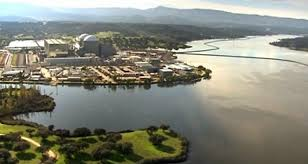
\includegraphics[width=0.47\textwidth]{2Introduction/ArrocampoDam.jpeg}}
  \subfloat[Tajus river along Spain and Portugal]{
   \label{fig:TajusRiver}
    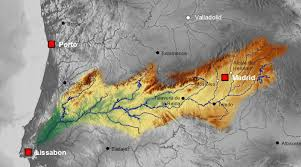
\includegraphics[width=0.53\textwidth]{2Introduction/RioTajo.jpeg}}
 \caption{Arrocampo dam, Almaraz NPP and Tajus river}
 \label{fig:Arrocampo}
\end{figure}

The \textit{Tritium} collaboration is a international group consisting of a consortium of 6 different southwestern european institution of 3 different countries: The University of Aveiro, in Portugal, The University of Bordeaux and the CNRS  (Section Aquitaine-Limousin), in France and the University of Extremadura, \textit{Junta de Extremadura} and University of Valencia, in Spain.

FOTOO TRITIUM

Each institution has focused in the development of a different part of all this project:
\begin{itemize}
\item{} First, the Extremadura group has developed and installed the ultra pure water system with wich we get water with very low conductivity, $\sigma \approx 10 ~\mu S / \cm$. The conductivity of the water before the cleaning proces is around $ 1000 ~\mu S / \cm$. This clean process is very important for two reasons. On the one hand, it is important for maintaining our detector very clean, which is a critical point. On the other hand, it's important because with this process we reduce the natural background since we remove several natural radiactive isotopes that there are in this water (except tritium) such as $\ce{^{222}Rn}$, $\ce{^{40}K}$ or $\ce{^{137}Cs}$. This system will be explained in the chapter \ref{chap:Ultrapure}.

\item{} Second, french group has develop the pasive shielding where our detector will work inside. It is based in ultra radiopure lead with very low intrinsic activity. The objective of this pasive shielding is to reduce the external natural background that affect to our system, for this reason we use lead. Obviously, this shielding doesn't have to affect to the measurement of our system, for this reason we use radiopure elements with very low intrinsic activity. This shielding will be explained in the chapter \ref{chap:Shields}, section \ref{sec:PasiveShields}.

\item{} Third, The Portugal and Spanish people has developed the simulations about this system. The program which we have used in this project is GEANT 4, which is a simulation package. It consiste in a extensive C++ library with which we can design the geometry of our detector, the physical processes which happen there, etc. This simulation will be explained in the chapter \ref{chap:Simulations}.

\item{} Lastly, The Portugal and Spain people has collaborated for designing, developing and building four different prototypes of tritium detector and active vetos for removing cosmic events. These prototypes and vetos will be explained in the chapter \ref{chap:Prototypes}.

\end{itemize}

The tritium level which we want to mesure follow the ALARA principle (As Low As Possible Achievable) and to get it there are important characteristics which our tritium detector must have:

\begin{itemize}

\item{} \textit{Compact}. This is important because in the place where this detector will be installed the useful space that we can use is finite.

\item{} \textit{Thin active volume and large active area}. On the one hand, we have to take into account that, as we have seen in the table \ref{MeanFreePathTritium} of the seccion \ref{sec:TritiumProperties}, the mean free path of the $\beta$ particle of tritium decay is very low so we need to work with thin active volumes. In the practice, Active thickness beyond the mean free path of the tritium will only contribute to the background. On the other hand, as we have checked in the seccion \ref{sec:StateOfTheArt} the efficiency of this type of detector scales with the active area so we need to design our detector with the largest possible active area.

\item{} \textit{High sensitivity to tritium}. We are going to work with low tritium activities so we need to reduce as much as possible the non-detected tritium events.

\item{} \textit{High specificity to tritium}. We need that our detector is able to distinguish the tritium signal of the signal of other radiactive elements which can be present in the initial sample.

\item{} \textit{Quasi-real time response}. As we have seen it is important that our sistem can work in quasi-real time in order to detect any problem as fast as possible. 

\item{} \textit{Rugged system}. Finally, we have to take into account that our objective will be installing an automatical system which will work during a lot of years without specialized people so we need that our monitor are rugged. 

\end{itemize}

In order to get the measurement in quasi-real time we need to work \textit{in situ}, that's, we need that our detector is able to work in the same place that we take the sample. Whit the work \textit{in site} we achieve:

\begin{itemize}
\item{} a faster monitor because we eliminates the process of taking the sample, the chain-of-custody until this sample arrive to this laboratory and the complexity which involve these tasks. 

\item{} a better monitor since if we can work \textit{in site}, our measurements can be more frequent hence we will can identify cahnges in the activity earlier.

\item{} a cheaper monitor because we have not only the material costs attached to the sample collection, chain-of-custody of this sample, shipping of this sample to the laboratory, etc. but we have also eliminated the costs attached to the specialized staff who are involving in these tasks. Our detector will only need frequent calibrations each time in order to ensure its correct operation.

\item{} a safer monitor since the personal exposure dose is reduced and the changes in activity are detected fastly. On top of that we remove the possibles mistakes which can be done by specialized staff.

\end{itemize} \label{sec:TritiumProject}
	\newpage
	
	\section{Work scheme}
	This thesis is build up as follow:...



The objetive of this three-phase project was design, develop and instalation and commisioning a automatical system capable of detection tritium which we find in the water that is used by the nuclear power plants for their cooling system. The initial idea was quantifying its activity in quasi-real time before discharging it into public rivers or seas. 

We are speaking all the time about getting the measurement in quasi-real time, that is, in less of 10 minuts but what about the real time? It is obviously imposible because we are mesuring the activity, I mean, we are counting tritium decays in samples with low activities (supposedly less than $100~\becquerel/\liter$) so we need some time in order to get enough stadistic with which we can distinguish the tritium signal to the background in our system.

In order to get the measurement in quasi-real time we need to work \textit{in situ}, that's, we need that our detector is able to work in the same place that we take the sample. The reason of this fact is because if we need to move the sample we lose a lot of time (1 or 2 days in some cases). Furthermore if we avoid to move the samples we get a:

\begin{itemize}
\item{} faster detector because we eliminates the process of taking the sample, the chain-of-custody until this sample arrive to this laboratory and the complexity which involve these tasks. 

\item{} better detector since if we can work \textit{in site}, our measurements can be more frequent hence we will can identify cahnges in the activity earlier.

\item{} cheaper detector because we have removed all the cost associated with the sample collection, chain-of-custody of this sample, shipping of this sample to the laboratory and analysis thereof there. Not only we have eliminated the material costs attached to this tasks (material, transport, etc) but we have also eliminated the costs attached to the specialized staff who are involving in these tasks. With our detector we will only need frequent calibrations each time, which we consider suitable, in order to ensure the correct operation of this detector

\item{} safer detector since the personal exposure dose is reduced and the changes in activity are detected fastly. On top of that we remove the possibles mistakes which can be done by specialized staff who follow each protocol of this tasks.

\end{itemize} 

Dividiremos este trabajo en seis partes:
\begin{enumerate}
\item{} En primer lugar, se realizará un estudio sobre las fibras centelleadoras para  determinar  el protocolo de manipulación para obtener un  procedimiento de preparación de  un haz de fibras centelleadoras con un buen rendimiento óptico. 

\item{} En segundo, lugar estudiaremos el procedimiento de calibración de los SiPM,  fundamental para el experimento.  No se necesita realizar una calibración de los PMT, paso igualmente importante al anterior, ya que este trabajo fue realizado recientemente por otro componente del grupo.

\item{} En tercer lugar, se describirá  el primer prototipo diseñado, formado por un haz de 35 fibras centelleadoras sin clad leídas por PMT,  incluyendo el protocolo del proceso de llenado con agua tritiada que tuvo que ser desarrollado para cumplir los requisitos de protección radiológica y evitar contaminación accidental,  y los  resultados obtenidos con el mismo.

\item{} En cuarto lugar, se presentarán las simulaciones realizadas con el programa de Geant4 en una configuración sencilla.

\item{} En quinto lugar, se expondrán aspectos a estudiar en el futuro inmediato y en etapas posteriores, durante la Tesis Doctoral. 


\item{} Se presentarán, finalmente, los resultados, logros y conclusiones alcanzadas en el desarrollo del  trabajo.

\end{enumerate}\label{sec:WorkScheme}
	\newpage
	
\chapter[Design principles]{Design principles of the Tritium monitor}\label{chap:DesignPrinciples}
	\section{Chapter scheme}
	This Chapter is divided in three different sections. First, we have a theorical explication about the interaction of fast electrons and photon with matter. Next, I show the main parts in which the TRITIUM detector consists. Finally, the foundamental explication and our own developments in scintillating fibers and photosensors are shown.
 \label{sec:IntroDesignPrinciples}
	\newpage

	\section[Interaction of particles with matter]{Interaction of fast electrons and photons with matter}
	In this section, the explanation will only focus on the particles and energy range that are interesting for this thesis, which are electrons ($0-18~\keV$) and photons in the visible range.

On the one hand, electrons have charge so their interaction with matter are mainly produced with the orbital electrons that there are in that matter, due to the Coulomb force. The trajectory which electrons follow is much more tortuous than other heavier particles because the mass of the interacting particles is equal, electrons. Furthermore, for the same reason, these electrons lost a significant amount of energy in each collision.

In order to speak about the total energy lost of particles in matter the specific energy loss is defined as $S=-\frac{dE}{dx}$ which expresses the energy loss suffered by the particle per unit of trajectory. In the case of electrons, this total energy loss has two main contributions, the collisions (elastic and inelastic) and radiative processes (bremsstrahlung):

$$\frac{dE}{dx} \approx \left(\frac{dE}{dx}\right)_{c} + \left(\frac{dE}{dx}\right)_{br} ~\cite{Knoll} \cite{Leo} \qquad  \frac{\left(\frac{dE}{dx}\right)_{br}}{\left(\frac{dE}{dx}\right)_{c}} \approx \frac{EZ}{700} ~\cite{Knoll}$$

Where $E$ is the energy of the electron in $\MeV$ and $Z$ is the atomic number of the absorbing material. Due to this energy loss, the electrons can only penetrate a material as far as they go before losing their total energy. This distance is known as range and, in the case of tritium electrons, its value is seen in the table \ref{MeanFreePathTritium}.

On the other hand, photons don't have charge. Its possible interactions with the matter are photoelectric effect, Compton effect, coherent scattering and pair production and the probability of each process depends on the energy of the photon, $E_\gamma = h\nu$, and the atomic number of the material, Z, as you can see in the figure \ref{ProcessesPhotons}.

\begin{figure}[htbp]
\centering
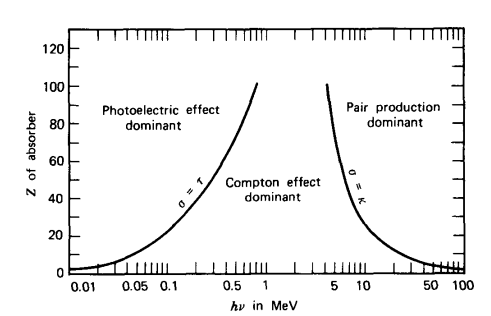
\includegraphics[scale=0.75]{3DesignPrinciples/DominantProcessesPhotons.png}
\caption{Domain regions of the three most probable types of interactions of gamma rays with matter. The lines show the values of Z and $h\nu$ where the two neighboring effects are equally likely.\label{ProcessesPhotons}~\cite{Knoll}~\cite{Leo}}
\end{figure}

We have to take into account that the only relevant photons for this thesis are in the visible range, between $400$ and $700~\nano\meter$, that corresponds with energies of the order of the $\eV$. Therefore the last effect, pair productions, will be not explained here because it needs a photon energy equal or more than $1.022~\MeV$ for happening and it is not our case.

The photoelectric effect occurs when a photon interacts with an orbital electron in the material, losing all its energy. This energy is absorbed by the electron that is released from the atom (ionization). The energy of the resulting electron is:

$$E_e = E_\gamma - E_b ~\cite{Knoll}\cite{Leo}$$

Where $E_e$ is the energy of the electron released and $E_b$ is the binding energy of the electron in this material. The probability of this effect depends on the number of available electrons through the variable Z, and the energy of the electron according to the following expression:

$$\left(Pr\right)_{Ph-eff} \approx \frac{Z^n}{E_\gamma^{3.5}}~\cite{Knoll}$$

As we can see in this expression and in the figure \ref{ProcessesPhotons}, the photoelectric effect is most probably if we use elements with high atomic number. This is the reason why elements with high atomic number are the best isulators against gamma radiation and this is the reason why we use lead ($Z=82$) for building our passive shielding as we will see in the section \ref{sec:PasiveShields}. 

The Compton effect occurs when the photon interacts with an orbital electron of the material, transferring part of this energy to the electron, which is released, and this photon is scattered at an angle $\theta$ with respect to the original direction. If we neglect the binding energy, the energy transfered to this electron, $E_e$, is shown in the following equation:

$$E_e=\frac{\frac{E_\gamma^2}{m_oc^2}\left(1-cos\theta\right)}{1+ \frac{E_\gamma^2}{m_oc^2}\left(1-cos\theta\right)}~\cite{Knoll}\cite{Leo}$$

Where $m_0$ is the rest mass of the electron and $c$ is the speed of the light in the vacumm. The probability of the Compton effect is proporcional to the atomic number(more available electrons), Z,  and decreases with the energy of the photon. 

As we can see in the figure \ref{ProcessesPhotons}, in the energies of the photons belonging to the visible range of the electromagnetic spectrum (of the order of eV), the Compton effect is only more likely in very light materials, (Z<4). For heavier materials the photoelectric effect is the dominant effect. This is the reason why we use elements with high number atomic in the cathode of the our PMTs.

Finally, in the coherent scattering, the atom is neither excitation nor ionization and the photon conserve all their energy in this collision. This effect is more probably for photons with low energies and materials with high atomic numbers.

Because of the fact that the energy of the photon doesn't change we will not speak more about this effect but it is important since this effect change de direction of photons and it will affect to their mean free path. \label{sec:Interaction}
	\newpage	
	
	\section[The detection process]{The detection process in a scintillation detector}
	Due to the reasons which we have discussed in the section \ref{sec:StateOfTheArt}, the type of the detector which we have developed in order to measure the tritium that there is in water samples is a scintillator detector. It consists in a chain of three main elements:

\begin{itemize}

\item{} The scintillator, that is the material in charge of detecting the tritium event. The tritium particle or a general particle (ionizing radiation) hit this material and deposits part of their kinetic energy (or all, as in the case of the tritium event) in it through ionization and excitation. Part of this energy deposited is converted in photons, in our case in the visible range.

The number of photons produced carry information about the particle detected, such as its energy, type, etc.

\item{} The photosensor, which is the part of the detector in charge of detecting the photons produced by the scintillator that reach its sensitive element (the more scintillated photons arrive to your photosensor, the better signal you have in your detector). 

The most used photosensor in nuclear physics are SiPMs and PMTs which detects some of the photons produced in the scintillator and transforms it in electrons which are multiplied with a factor of around $10^6$. This millions of electrons form a electronic pulse whose properties has information of the photons that has been detected.

\item{} The electronic system, which is the part of the scintillator detector in charge of processesing and analyzing (first analogically and then digitally) this electrical pulse of the photosensor to give us useful information about the event detected that we can understand and interpret such as a number, for instance the activity, or some kind of spectrum like energetic spectrum.

\end{itemize}

In figure \ref{fig:ScintillatorDetector} we can see the scheme of a scintillation detector where the scintillator material detects ionizing radiation and produces photons that will be guided by the reflector and the light guide to the photosensor. There, some of the photons that reach the sensible part of the photosensors will be converted and multiplied into millions of electrons that will form a electronic pulse. The output signal of the photosensor (electronic pulse) will be processed and analyzed by the corresponding electronics:

\begin{figure}[hbtp]
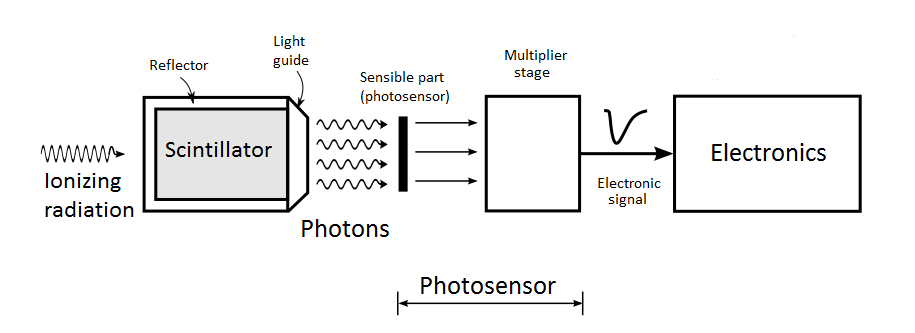
\includegraphics[scale=0.6]{3DesignPrinciples/ScintillatorDetector.png}
\centering
\caption{Scheme of the scintillator detector \cite{CentelleadoresEspanyol}\label{fig:ScintillatorDetector}}
\end{figure} \label{sec:DetectionProcess}
	\newpage
	
	\section{Scintillators plastic} %\label{sec:Scintillators}
	The use of scintillators in radiation detection is one of the most used technics in nuclear physics. The scintillator is a material that is able to convert the kinetic energy of the incoming particles in light (photons in the visible energy range) which we can detect and quantify. It happens because the radiation excites and ionizes the scintillating atoms which, after that, are immediately de-exciting (with times of the order of picoseconds), emitting photons.

This conversion should be linear in a wide energy range of incoming particles and it is necessary that this material has good optical properties, such as being transparent to the wavelenght of their own emission and having a refractive index as close as possible to the glass for optimizing optical coupling with photosensors.

The photon emission in the scintillator is a stadistical process, which means that two exactly the same events will emmit different number of photons. It follow a poisson statistics so when we speak about the number of emmited photons we speak about the mean number of photons.

There are two types of scintillators, organics and inorganics. Inorganic scintillators normally have a higher atomic number and density so their light output are higher. Due to these reasons they are better for gamma-ray spectroscopy (take into account figure \ref{ProcessesPhotons}). Organic scintillators generally are faster and they are commonly used for beta spectroscopy and neutron detection. In this seccion I focus my explanation mainly on organic scintillators since they are the ones we have used in our research. 

Organic scintillators are based on a scintillator material, which produces light, dissolved in a base solvent. This solvent is normally based on aromatic hydrocarbons (carbon atoms linked together), that is, they are mainly composed of carbon and hydrogen atoms as we can see in the molecules of some of the most widely used scintillators, $\ce{C_{18}H_{14}}$, $\ce{C_{24}H_{22}N_{2}O}$ or $\ce{C_{15}H_{11}NO}$ whose average atomic numbers are between 3,5 and 5.

The scintillator molecules, in which the organic scintillators are based, have the so called $\pi$-electron structure. The energy levels of their electrons are commonly ilustrated with a Jablonsky diagram, figure \ref{JablonskyDiagram}, where we can see the fundamental single state, $S_{0i}$, where the valence electrons are, the excited single states, $S_{jk}$, and the excited triple states, $T_{lm}$. De energy difference between $S_1$ and $S_0$ states is around $3$ or $4~\eV$, energy range of the visible photons. We can see in this diagram that each of this energy states are subdivided in smaller energetic sublevels whose distance between them are around $0.15~\eV$. This finer energy structure is due to the excitations of molecular vibrational modes and they are expresed with the second index of the energy states.

\begin{figure}[htbp]
\centering
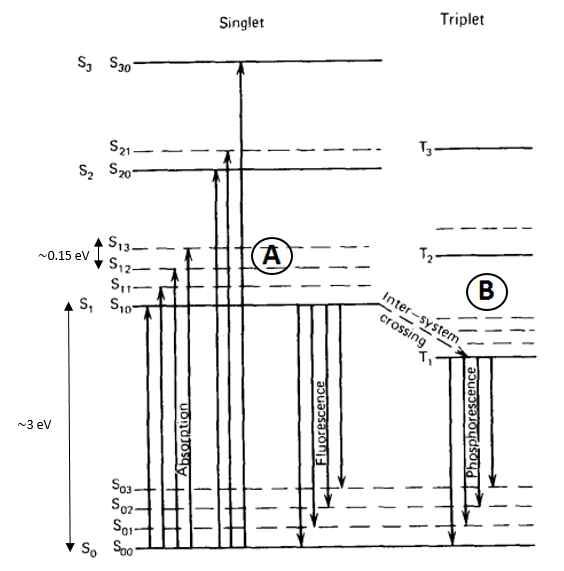
\includegraphics[scale=0.6]{3DesignPrinciples/JablonskyDiagram.png}
\caption{Jablonsky diagram.\label{JablonskyDiagram}~\cite{Knoll}}
\end{figure}

Because of the reason that the distance between all energy levels and sublevels are larger than the termal energy, $0.025~\eV$, non-exciting electrons are in the lowest state $S_{00}$ at standar temperature conditions.

When a particle deposits their kinetic energy on a scintillator, their valence electrons are exited to higher single energetic states very fast (times of the order of picoseconds) which is expressed with upwards direction arrows in the figure \ref{JablonskyDiagram} and they are quickly de-excited to the first single excited state, $S_{10}$, through non-radiactive processes known as internal conversion.

Now, this electrons can de-excited to the fundamental single state, $S_{00}$, through three different physical mechanisms:

\begin{itemize}

\item{} The prompt fluorescence(process A in figure \ref{JablonskyDiagram}), where the electron in the $S_{10}$ energy level  is de-excited to some sublevel of the fundamental state $S_{0i}$, emitting a photon with an energy equal to the energy difference of these levels (around $3~\eV$, visible light). This process happens immediately after the excitation of the scintillator molecules (around tens of nanoseconds after excitation). Each scintillator has a characteristic emission spectrum that defines its response due to the fluorescence mechanism. 

Now we can understand why organic scintillators are practically transparent to their own fluorescense emission. This is because of the reason that there existe a quenching effect in each de-excitation process whereby there are a lost of radiated energy. Due to that, all emmited  photons by the scintillator have less energy than the required energy for excitation. This effect is called Stokes shift and it's represented with a general wavelenght spectrum in the figure \ref{StokesShift}.

\begin{figure}[htbp]
\centering
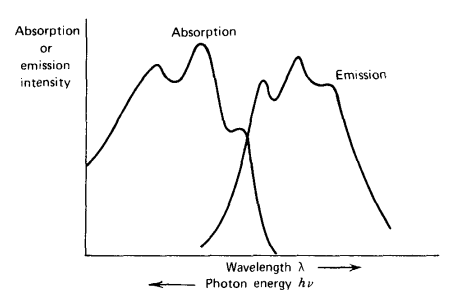
\includegraphics[scale=0.7]{3DesignPrinciples/StokesShift.png}
\caption{Stokes shift.\label{StokesShift}~\cite{Knoll}}
\end{figure}

One of the most important parameters in nuclear physics is the scintillation yield, whcih is the fraction of particle energy that is converted in light. All mechanisms which don't produce prompt fluorescence, like phosphorescence or delay fluorescence, which we will see later, or even internal conversion, contribute to reduce this parameter. The signal of the scintillator depends on the type of particle so, the scintillation yield will be different. This factor is normally given by the manufacturer for mips (minimum ionized particles, that's, for example, electrons with $500~\keV$ or more) in number of photons per $\MeV$.

The intensity of the fluorescence emission in an organic scintillator during time is a combination of two exponential functions, one associated with the lifetime of the level, $\tau$ (on the order of nanoseconds), and the other associated with the energetic level population, $\tau_1$ (on the order of picoseconds).

$$I=I_0\left(e^{t/\tau} - e^{t/\tau_1}\right) \cite{Knoll}$$

\item{} The phosphorescence, where the electron, which is in the first single excited state, cross to a triple excited state (process B in figure \ref{JablonskyDiagram}) with a process called "intersystem crossing". This is a metastable state with a much longer lifestime so electrons in this state are de-excited to the $S_{0i}$ state, emitting a photon much later than phosphorescence. This process can happen up to $10^{-3}$ seconds after scintillator excitation.

\item{} Delayed fluorescence, which occurs when an electron is in a triple excited state but whose transition to the ground state is forbidden. In this case, this electron can interact with another in the same state and return to the first single state ($S_{1}$ is more energetic level than $T_{1}$) and quickly de-excited to the ground state. 

$$T_{1} ~+~ T_{1}~ \longrightarrow ~ S_{1} ~+~ S_{0} ~+~ phonons$$

This emission has the same emission spectrum as immediate fluorescence, but occurs later.

\end{itemize}

The scintillating detectors generally use the prompt fluorescence light as output signal so a good scintillator should increase it and reduce other possible physical mechanisms.\label{sec:PlasticScintillators}
		
		\subsection{Plastic scintillation fibers}
		Plastic scintillators are organic scintillators that has been disolved in a solven and polimerized. They are easy to machine and can take any desired shape during construction. Among the forms most used today we can find blocks, thin sheets, cylinders, etc.

In our experiment we have been working with an plastic scintillator in the form of fiber, specifically, commercial fibers BCF-12 from Saint-Gobain Crystals Inc \cite{DataSheetBCF12Fiber}. This type of fiber was chosen as the result of a comparative study among some of the best-known commercial manufacturers, such as Kuraray. 

The BCF-12 fibers consist of a scintillated core, whose material is polystyrene, one of the most used solvents for plastic scintillators \cite{Knoll}, with the posibility of surounding it of a cladding of polymethylmethacrylate (PMMA) (smaller refractive index than core in order to archieve a critical angle) or a multicladding (second cladding) with even smaller refractive index.

When a particle deposits all or part of its kinetic energy, some photons are produced in the fiber core as a result of the scintillating process. The quantity of photons which are produced depend on the scintillation yield, whose value is around $8000$ photons per $\MeV$ from a minimum ionizing particle in our case (BCF-12 fibers) . It means that, for instance, for tritium electron, this fibers will release a maximum of around 148 photons (when tritium electron has the maximum energy, $18.6~\keV$).

These photons will shape the useful part of the response of the scintillator (fluorescence) for us. The energy (or wavelength) of these scintillated photons follows the distribution of their emission spectrum which, for the used fibers, is shown in the figure \ref{EmissionSpectrumFibers}.

\begin{figure}[htbp]
\centering
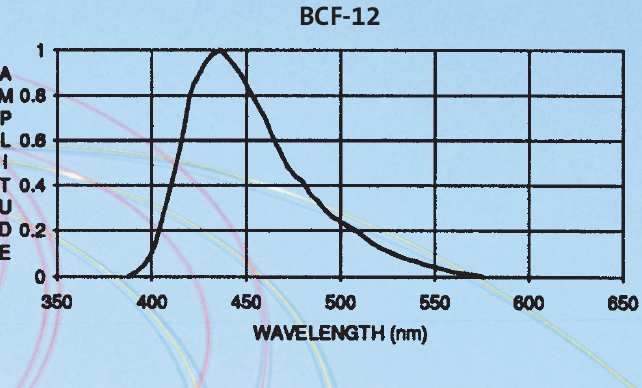
\includegraphics[scale=0.5]{3DesignPrinciples/EmisionBCF12.png}
\caption{Emission spectrum of BCF-12 fibers of Saint-Gobain.\label{EmissionSpectrumFibers}~\cite{DataSheetBCF12Fiber}}
\end{figure}

After the production of scintillated photons, we need to guide these photons to the sensitive part of the photosensor where we will detect them with some probability. Fibers (and scintillators in general) use the optical property of Snell's law \ref{} to guide their photons to the desired part (the ends of the fibers). It is based on the interface created between the core and the surrounding material. When a photon hits this interface, it is refracted (and therefore lost) following the Snell equation, \ref{}. If the surrounding material has a lower index of refraction than the core of the fiber, there exist a critical angle, $\theta_c$, at which, for angles equal or larger than this one, the photons will be totally refracted (and therefore conserved in the fiber for being guided).

$$n_0~sen(\theta_0) = n_1~sen(\theta_1) \longrightarrow \theta_c = asen\left(\frac{n_1}{n_0} \right)$$

There exist a parameter which define the efficiency of the scintillator in order to guide photons, the trapping efficiency. For BCF-12 fibers is between $3.44\%$ and $7\%$ (depending if the event was detected near the fiber axis (minimum) or near the core-clad interface(maximum)).

Therefore, from these $148$ photons initially created with the tritium electron with the maximum energy, only a maximum of around 10 photons (for maximum trapping efficiency) will arrive to our photosensor. As you can see, we work with very weak electronic signals, where there is more electronic noise and, as you will see in future chapters, we have made a big effort to reduce this electronic noise as much as possible with several technics.

In the figure \ref{Fiber_physic} we can see how a scintilalting fiber works.

\begin{figure}[htbp]
\centering
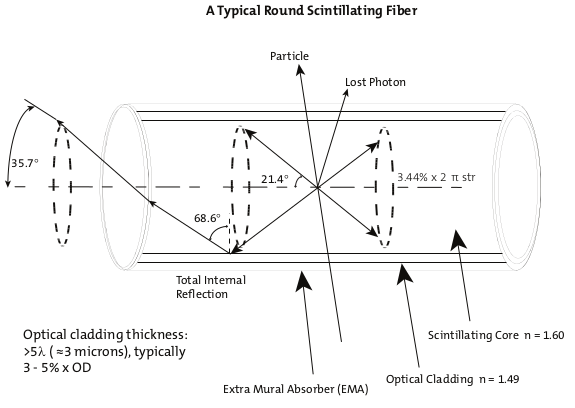
\includegraphics[scale=0.5]{3DesignPrinciples/Fiber_data_sheet.png}
\caption{How photons are collected in a fiber with single clad.\label{Fiber_physic}~\cite{DataSheetBCF12Fiber}}
\end{figure}

The cladding material is useful for protecting the core surface from dirt or aggressive external agents what can reduce the light collection but at the cost of losing some light because it increase the critical angle. In the table \ref{tab:CriticalAngles} we have three different examples where this effect is ilustrated.

\begin{table}[htbp]
%%\centering
\begin{center}
\begin{tabular}{|c|c|c|}
\hline
Material & Refractive index & critical angle ($\degree$) \\
\hline \hline \hline
Air & 1 & $42.98$ \\ \hline
Water & 1.33 & $62.47$ \\ \hline
Cladding of PMMA & 1.49 & $76.26$ \\ \hline
\end{tabular}
\caption{Critical angles asociated to different interfaces created with polystyrene, $n_0=1.6$, and other materials}
\label{tab:CriticalAngles}
\end{center}
\end{table}

This is what theoretically happens but, in the practice, it's difficult to archieve a perfect air-core or water-core interface and it will affect to the light collection. Due to the reason that the commercial claddings are thicker ($30~\micro \meter$) than the mean free path of tritium in water ( around $5~\micro\meter$) we cannot use cladding in our detector hence we will need to take special attencion for archieving a water-core interface enough good.

Some of the most important properties of the used fibers are shown in the table \ref{tab:ParametersFibersBCF12}.

\begin{table}[htbp]
%%\centering
\begin{center}
\begin{tabular}{|c|c|c|}
%\hline
%Material & Refractive index \\
\hline \hline 
Core material & Polystyrene \\ \hline
Core refractive index & 1.60 \\ \hline
Density & 1.05 \\ \hline
Cladding material & Acrylic (PMMA) \\ \hline
Cladding refractive index & 1.49 \\ \hline
Cladding thickness ($\mu\meter$) & 30 \\ \hline
Numerical aperture & 0.58 \\ \hline
Trapping efficiency & 3.44\% minimum \\ \hline
No. of H atoms per cc (core) & $4.82 \cdot{} 10^{22}$ \\ \hline
No. of C atoms per cc (core) & $4.85 \cdot{} 10^{22}$ \\ \hline
No. of electrons per cc (core) & $3.4 \cdot{} 10^{23}$ \\ \hline
Radiation lenght (cm) & 42 \\ \hline
Emission peak (nm) & 435 (Blue) \\ \hline
Decay Time, (ns) & 3.2 \\ \hline
1/e Length (m) & 2.7 \\ \hline
Scintillator yield (\#$\gamma$/MeV) & $\sim 8000$ \\ \hline
Operating Temperature & $-20\degree C$ to $50\degree C$ \\ \hline
\end{tabular}
\caption{Properties of BCF-12 fibers from Saint-Gobain Inc. \cite{DataSheetBCF12Fiber}}
\label{tab:ParametersFibersBCF12}
\end{center}
\end{table}

%Bunch -> manojo de fibras

%bundle -> haz de fibras\label{subsec:PlasticScintillatorFibers}
		\newpage
		
	\section{The light process in photosensors} %\label{sec:Photosensors}
	So far we have created the scintillating photons in the core of the fiber, which has been guided to its ends. Now, what we need is the so-called photosensor, which is an element that is able to detect these scintillating photons. Photosensors have a sensitive part that is optimized to detect photons in a range of energies (normally inside of a visible range) with enough efficiency. After that, the photosensors create an electronic signal that carries information about these detected photons, such as their number or their detection time.

One of the most important things in the scintillation detector is that the emission spectrum of the scintillation (figure \ref{EmissionSpectrumFibers}) overlaps as much as possible with the detection efficiency spectrum of the photosensor used, specifically their maximums. In this case, the efficiency of this detector,  which is poroporcional to the multiplication of both factors at the same photon energy, will be optimized (the largest).

There are a lot of different photosensors that can be used for this purpose, whose photon detection relies on totally different physical processes, such as photoelectron multiplier tubs (PMTs), silicon photoelectron multiplier (SiPM) or charge-coupled device (CCD).  Each one of these will have different properties and we have to choose the one which fit better for our objective.

Our main proposal for our scintillation detector will be to use SiPM arrays because they are very fast (of the order of $~\nano\meter$) and have high photodetection efficiency (a maximum of around $50\%$) and multiplication faction ($10^{6}$). On top of that, one of the most important reason of this choice is that SiPM arrays are able to detect a single photon, which is very important since, as we have seen in the seccion \ref{subsec:PlasticScintillatorFibers}, just a few photons will arrive to the sensible part of the photosensor. We will test also the PMTs, which are the conventional choice, because they are still interesting since they have lower dark count rate than equivalent SiPM.




%A certain portion (in an optimal case nearly 100\%) of the scintillation photons reach the light detector, which has to be sensitive enough to detect a small number of photons. The detector then produces a signal pulse, which has a height proportional to the number of photons hitting the detector. The signal pulse of the detector is processed by the electronics, and as a result a pulse height spectrum is produced (see Section 3.5).

%This spectrum corresponds to the energy spectrum of the detected particles.


%such as their height or their time, is related with information about the photons such as their number or their time.\label{sec:Photosensors}
	
			\subsection{Photoelectron multiplier Tubs (PMTs)}%\label{subsec:PMTs}
			Photoelectron multiplier tube is one of the most used photosensors in nuclear physics during last decades. Its main objective, like all photosensors, is to detect the scintillating photons that reach its sensible part and covert it in an electronic signal large enough to be measured. The way in which PMTs achieve this objective is based in two different phases:

\begin{itemize}
\item{} First, the PMT convert photons that reach its sensible part in electrons with some probability. The sensible part is the photocathode (sensible part of the PMT) which consists in a fina capa de un material que produzca efecto photoelectrico con grán probabilidad. En nuestro caso el material utilizado es. La probabilidad de... es... el espectro de emission...  

- Hablar del photocatodo, parte sensible bla, bla, bla. Espectro de efficiencia, función de trabajo del photocatodo, etc...

\item{} After that, secondary electron multiplication

- Hablar de la etapa de ganancia, dinodos, circuito electrónico divisor de ganancia, bla, bla bla...

2 circuitos diferentes. En principio equivalentes pero el primero más seguro y el segundo mejor para mediciones precisas de tiempo y de alta tasa de cuentas.

\end{itemize}


Cuando acabe con todo esto hablar del resto de elementos, tubo de vacío, etc...


The PMT has two main functions. On the one hand it is able to convert photons, whose energy are inside of a energy range, in electrons throgh photoelectric effect. On the other hand, it capable of multiplying these electrons with high gain factors.


an electric pulse. It is based on a photocathode, which is the sensible part of the photosensor. The photocathode release an electron with some probability when a photon reach it...

IMAGEN

Nuestros objetivos para elegir el PMT y SiPM adecuado.

Leer el capitulo de PMTs del trabajo de "Centelleadores" -> Clave para explicar estas 2 etapas.

Leer el capitulo de PMTs de la tesis de fibras
Leer el capitulo de PMTs de la tesis alemanan -> Clave para los elementos externos, tubo de vacío, etc.



Linear response with the incoming photons.



Incluir lo de la intro de photosensores

%Conceptualmente, un fotomultiplicador cuenta con un fotocátodo y un multiplicador de electrones. El primero es una fina capa de un compuesto que emite electrones cuando absorbe fotones en el espectro visible o en las cercanı́as de él. Los electrones emitidos por el fotocátodo son llamados fotoelectrones. El segundo, de nombre sugestivo, es un arreglo de electrodos conectados a alta tensión que permite obtener ganancias de 10 6 . Más adelante en este capı́tulo, volveremos sobre los PMT.

\label{subsec:PMTs}
			%\newpageand
		
			\subsection{Silicon Photoelectron Multiplier Array (SiPMs array)}%\label{subsec:SiPMs}
			MPPC Multi-Pixel Photon Counter

Linear response with the incoming photons.

Ver apuntes generales comentados de photosensores en la intro de photosensores

Los tubos fotodetectores (PMT) son los dispositivos adecuados para esto, aunque, sin embargo, los avances tecnologicos de las ultimas decadas en tecnologia de semiconductores ha permitido el desarrollo de los fotodiodos de avalancha operados en modo Geiger (APD, Avalanche PhotoDiode)

Actualmente, la tecnologia de semiconductores ha permitido el desarrollo de fotodiodos que, por sus prestaciones, pueden reemplazar adecuadamente a los PMT. \label{subsec:SiPM}
			%\newpage
			
			\subsection[Comparison photosensors]{Comparison of photosensors considered}%\label{subsec:SiPMs}
			\input{./Sections/3Design_Principles/34Photosensors/343Comparison_Photosensors}\label{subsec:ComparisonPhotosensors}
			\newpage
		
	\section{Detector pulse analysis}%\label{sec:PulseAnalysis}
	\input{./Sections/3Design_Principles/35Pulse_Analysis}\label{sec:PulseAnalysis}
	\newpage
	
	\section{Tritium monitor parts}%\label{sec:PulseAnalysis}
	\input{./Sections/3Design_Principles/36Tritium_Monitor_Parts}\label{sec:TritiumMonitorParts}	
	\newpage
	
\chapter[Research \& Development]{Research \& Development on detector design and components}\label{chap:ResearchandDevelopment}
	\section{Introduction (why is important)}
	%\input{./Sections/3ResearchAndDevelopment/3IntroductionChapter} \label{sec:IntroChap}
	\newpage
	
	\section[Characetrization fibers]{Characterization and R\&D on scintillating fibers}
	%\input{./Sections/3ResearchAndDevelopment/33ScintillatingFibers/332RyD_SF}\label{subsec:RyDSF}
	\newpage
		
	\section[Characterization SiPM arrays]{Characterization and R\&D on the SiPM arrays}
	%\input{./Sections/3ResearchAndDevelopment/34Photosensors/342SiliconPhotoMultiplier/3422RyD_SiPM}\label{subsubsec:RyDSiPM}
	\newpage

\chapter{Tritium monitor prototypes}\label{chap:Prototypes}		
	\section[Preliminary prototypes]{Preliminary prototypes, TRITIUM-IFIC 0, TRITIUM-IFIC 1 and TRITIUM-Aveiro}\label{Preliminary_prototypes}
		\subsection{Tritium-IFIC 0}
		%\input{./Sections/4Prototypes/41TritiumIFIC0}\label{subsec:TritiumIFIC0}
		%\newpage
		
		\subsection{Tritium-IFIC 1}
		%\input{./Sections/4Prototypes/42TritiumIFIC1}\label{subsec:TritiumIFIC1}
		%\newpage
		
		\subsection{Tritium-Aveiro}
		%\input{./Sections/4Prototypes/43TritiumAveiro}\label{subsec:TritiumAveiro}
		\newpage
		
	\section[Tritium-IFIC 2]{Advanced prototype, Tritium-IFIC 2}
	%\input{./Sections/4Prototypes/44TritiumIFIC2}\label{sec:TritiumIFIC2}
	\newpage
		
	\section[Modular TRITIUM prototype]{Modular TRITIUM prototype for in-situ tritium monitoring}
	%\input{./Sections/4Prototypes/45TritiumIFICMonitor}\label{sec:TritiumMonitor}
	\newpage
		
\chapter[Background shields]{Tritium monitor background shields}\label{chap:Shields}
	\section{Tritium monitor background}
	%\input{./Sections/5Shields/51IntroductionShields}\label{sec:IntroductionShields}
	\newpage
		
	\section{Passive shield (lead)}
	%\input{./Sections/5Shields/52PasiveShields}\label{sec:PasiveShields}
	%\newpage
		
		\subsection{Introduccion}
		%\input{./Sections/5Shields/52PasiveShields}\label{sec:PasiveShields}
		%\newpage
		
		\subsection[Set up of the shield]{Set up of the Passive shield}
		%\input{./Sections/5Shields/52PasiveShields}\label{sec:PasiveShields}
		%\newpage
		
		\subsection[Measurements of the shield]{Measurements with the passive shield}
		%\input{./Sections/5Shields/52PasiveShields}\label{sec:PasiveShields}
		\newpage	
	
	\section{Active shield (cosmic veto)}
	%\input{./Sections/5Shields/53ActiveShields}\label{sec:ActiveShield}
	%\newpage
	
		\subsection{Introduccion}
		%\input{./Sections/5Shields/52PasiveShields}\label{sec:PasiveShields}
		%\newpage
		
		\subsection[Set up of the shield]{Set up of the active shield}
		%\input{./Sections/5Shields/52PasiveShields}\label{sec:PasiveShields}
		%\newpage
		
		\subsection[Measurements of the veto]{Measurements with the active shield}
		%\input{./Sections/5Shields/52PasiveShields}\label{sec:PasiveShields}
		\newpage
	
\chapter{Ultrapure water system}\label{chap:Ultrapure}
	\section{Introduction}
	%\input{./Sections/6Shields/61IntroductionUltraPure}\label{sec:IntroductionUltrapure}
	\newpage
	
	\section[Set up of water system]{Set up of the ultrapure water system}
	%\input{./Sections/6Shields/62SetupUltraPure}\label{sec:SetupUltrapure}
	\newpage
	
	\section[Measurements of water system]{Measurements of the ultrapure water system}
	%\input{./Sections/6Shields/63ResultsUltraPure}\label{sec:ResultsUltrapure}
	\newpage
	
\chapter{Electronical system}\label{chap:Electronic}
	\section{Introduction}
	%\input{./Sections/6Shields/61IntroductionUltraPure}\label{sec:IntroductionUltrapure}
	\newpage
	
	\section[Electronical system for PMTs]{Electronical system for PMTs}
	%\input{./Sections/6Shields/62SetupUltraPure}\label{sec:ElectronicaPMTs}
	\newpage
	
	\section[PETSYS (SiPMs)]{Electronical system for SiPMs arrays (PETSYS) }
	%\input{./Sections/6Shields/63ResultsUltraPure}\label{sec:PETSYS}
	\newpage
	
\chapter[Results and discussion]{TRITIUM Monitor results and discussion}\label{chap:Results}
	\section{Results from laboratory measurements}
	%\input{./Sections/7Results/71Results_prototypes}\label{sec:ResultsPrototypes}
	\newpage
		
	\section{Results from measurements at Arrocampo dam}
	%\input{./Sections/7Results/72ResultsArrocampo}\label{sec:ResultsArrocampo}
	\newpage	

\chapter{Simulations}  \label{chap:Simulations}
%\input{./Sections/8Simulations}
\newpage	

\chapter{Conclusions and prospects}  \label{chap:Conclusions}
%\input{./Sections/9Conclusions}
\newpage


\appendix
\appendixpage
\noappendicestocpagenum
\addappheadtotoc

\chapter{Birks coefficient study}\label{App:Birks}
Aún faltan cosas por decir.

\chapter{Más cosas}\label{App:A}
Aún faltan cosas por decir.

\chapter{Y más cosas aún}\label{App:B}
Y más cosas aún.

%\chapter{Bibliografía} \label{chap:bibliographia}
%\section {Bibliografía}
\begin{thebibliography}{100}
%Reference 1
\bibitem{Renovables} \textsc{F. J. Echarte},
\textit{El futuro de las energías renovables en España}, Universidad de Navarra, \href{https://tecnun.unav.edu/alumni/compartiendo-experiencia/futuro-energias-renovables}{\textbf{TECNUN'01 IESE'13}}.

%Reference 2
\bibitem{EIA}
\textit{International Energy Outlook 2013}, \href{https://www.eia.gov/outlooks/ieo/}{\textbf{U. E. Energy Information Administration}}.

%Reference 3
\bibitem{HighestCO2}
\href{https://news.un.org/en/story/2019/11/1052111}{\textbf{UN news}}, Global prespective Human stories

%Reference 4
\bibitem{Kyoto}
\textit{Kyoto protocol and reference manual}, 2008, \textbf{United Nations}.

%Reference 5
\bibitem{ITER}
\href{https://www.iter.org/}{\textbf{ITER}}, International Thermonuclear Experimental Reactor.

%Reference 6
\bibitem{TritiumDocument} \textsc{A. Fiege}, 
\textit{Tritium}, Kernforschungszentrum Karlsruhe, \textit{1992}.

%Reference 7
\bibitem{FusionCourse} \textsc{Eduardo Oliva Gonzalo}, \textsc{Adriana Ortiz Gómez}, \textsc{Nuria Moral Fernández}, \textsc{Alejandro Carrasco Sánchez}, \textsc{José Manuel Perlado Martín}, \textsc{Raquel Suárez Hontoria}, \textsc{Manuel Cotelo Ferreiro} 
\textit{Curso Básico de Fusión Nuclear}, jóvenes nucleares, Sociedad Nuclear Española, \textit{Septiembre de 2017, Madrid, Spain}.

%Reference 8
\bibitem{ComparationEmissions} \textsc{Benjamin K. Sovacool},
\href{https://www.academia.edu/2639807/Valuing_the_greenhouse_gas_emissions_from_nuclear_power_A_critical_survey}{\textit{Valuing the greenhouse gas emissions from nuclear power: A critical survey}}, ELSEVIER, Energy Policy  \textit{Vol 36} p. 2940-2953.

%Reference 9
\bibitem{PercentageEnergySpain}
\href{https://www.ree.es/es/datos/publicaciones/informe-anual-sistema/informe-del-sistema-electrico-espanol-2019}{\textit{Avance del informe del sistema eléctrico español, 2019}}, 
\textbf{Red eléctrica española}.

%Reference 10
\bibitem{ThreeMileIsland}
\href{www.world-nuclear.org/information-library/safety-and-security/safety-of-plants/three-mile-island-accident.aspx}{\textit{Three mile island accident}}, \textbf{World Nuclear Association}.

%Reference 11
\bibitem{CloseNPP}
\href{https://cincodias.elpais.com/cincodias/2018/11/15/companias/1542275699\_182457.html}{\textit{Cierre de centrales nucleares en España antes de 2030}}, \textbf{Cinco Días, El Pais}.

%Reference 12
\bibitem{60ReactorsChina}
\href{https://www.europapress.es/internacional/noticia-china-construira-menos-60-centrales-nucleares-proxima-decada-20160916210159.html}{\textit{China construirá 60 centrales nucleares en la próxima década}}, 
\textbf{Europa press}.

%Reference 13
\bibitem{35MillionsUSA}
\href{https://www.energynews.es/estados-unidos-centrales-nucleares/}{\textit{Inversión de EE. UU. de 35 millones para centrales nucelares}},\textbf{Energy News}.

%Reference 14
\bibitem{FiberDetector1a} \textsc{J. W. Berthold}, \textsc{L. A. Jeffers},
\href{https://www.osti.gov/biblio/2225-phase-final-report-situ-tritium-beta-detector}{\textit{Phase 1 Final Report for In-Situ Tritium Beta Detector}}, 
U. S. Department of Energy, McDermott Technology, Inc.,Research and Development Division, 	\textbf{DE-AC21-96MC33128}, April, 1998.

%Reference 15
\bibitem{FiberDetector1b} \textsc{J. W. Berthold}, \textsc{L. A. Jeffers}, 
\href{https://www.osti.gov/biblio/836625-MxOOUa/native/}{\textit{In Situ Tritium Beta Detector}}, U. S. Department of Energy, McDermott Technology, Inc. (MTI), Technology development data sheet, \textbf{DE-AC21-96MC33128}, May, 1999.

%Reference 16
\bibitem{CommonEmissionTritium} \textsc{X- Hou},  
\textit{Tritium and \ce{^{14}C} in the environmental and nuclear facilities: Sources and analytical methods}, Journal of the Nuclear Fuel Cycle and Waste Technology (JNFCWT), 16 (2018), 11-39 \href{https://doi.org/10.7733/jnfcwt.2018.16.1.11}{\textbf{DOI: 10.7733/jnfcwt.2018.16.1.11}}.

%Reference 17
\bibitem{FERMILAB}
\href{https://www.fnal.gov/pub/tritium/}{Tritium at Fermilab}.

%Reference 18
\bibitem{BrookHavenNationalLaboratory}
\href{https://www.bnl.gov/hfbr/decommission.php}{\textbf{Brookhaven National Laboratory (BNL)}}.

%Reference 19
\bibitem{TrackingTritium} \textsc{Aleksandra Sawodni}, \textsc{Anna Pazdur}, \textsc{Jacek Pawlyta}, 
\href{http://yadda.icm.edu.pl/baztech/element/bwmeta1.element.baztech-article-BAT3-0035-0005}{\textit{Measurements of Tritium Radioactivity in Surface Water on the Upper Silesia Region}}, Journal on Methods and Applications of Absolute Chronology, Geochronometria, Vol. 18, pp 23-28 \textbf{2000}.

%Reference 20
\bibitem{100BqL}  
\href{https://eur-lex.europa.eu/eli/dir/2013/59/oj}{\textit{Council directive 2013/15/euratom}}.

%Reference 21
\bibitem{740BqL} \textsc{Title 40},  
\href{https://www.ecfr.gov/cgi-bin/text-idx?node=pt40.1.141}{\textit{Protection of the Environment, US Code of Federal Regulations}} Part 141, Section 66, June 2011, \textbf{e-CFR (Electronic Code of Federal Regulations)}.

%Reference 22
\bibitem{CrossSeccionNeutrons}  
\textit{REFERENCIAAAAAAAA}.

%Reference 23
\bibitem{TritiumDiscovery} \textsc{M. L. Oliphant}, \textsc{P. Harteck} and \textsc{E. Rutherford},  
\href{https://royalsocietypublishing.org/doi/10.1098/rspa.1934.0077}{\textit{Transmutation Effects observed with Heavy Hydrogen}}, Nature, 133, 413 (1934)\href{https://doi.org/10.1038/133413a0}{\textbf{DOI: 10.1038/133413a0}}.

%Reference 24
\bibitem{TritiumIsolate} \textsc{Luis W. Alvarez} and \textsc{R. Cornog},  
\textit{Helium and Hydrogen of Mass 3}, Physical Review Journals Archive, 53, 613 (1939)\href{https://doi.org/10.1103/PhysRev.56.613}{\textbf{DOI: 10.1103/PhysRev.56.613}}.

%Reference 25
\bibitem{TritiumHandling} 
\href{https://www.twirpx.com/file/1977676/}{\textit{DOE Handbook: Primer on Tritium Safe Handling Practices}}, U. S. Departament Of Energy Washington, D.C. 20585.

%Reference 26
\bibitem{OxigenTritium} \textsc{Robert Haight}, \textsc{Joseph Wermer} and \textsc{Michael Fikani},
\textit{Tritium Production by Fast Neutrons on Oxygen: An Integral Experiment}, Journal of Nuclear Science and Technology, 39:sup2, 1232-1235, \href{https://doi.org/10.1080/00223131.2002.10875326}{\textbf{DOI: 10.1080/00223131.2002.10875326}}. 

%Referencia 27
\bibitem{CrossSeccionNeutrino} \textsc{},
\textit{REFERENCIAAAA}, \textbf{}

%Referencia 28
\bibitem{TritiumDecayEnergyLevels} 
\href{https://www-nds.iaea.org}{\textit{International Atomic Energy Agency}}.

%Referencia 29
\bibitem{TritiumDecayImage} 
\href{https://conexioncausal.wordpress.com}{\textit{Tritium decay image}}.

%Referencia 30
\bibitem{TesisTritio} \textsc{Zoltán Köllo},
\href{https://publikationen.bibliothek.kit.edu/1000049424}{\textit{Tesis: Studies on a plastic scintillator detector for activity measurement of tritiated water}}, Facultad de Física, Instituto Tecnológico de Karlsruhe (KIT), Karlsruhe, Alemania, \textit{17/07/2015}, \textbf{DOI: 10.5445/IR/1000049424}

%Referencia 31
\bibitem{AutoRadyolisis} \textsc{Sylver Heinze}, \textsc{Thibaut Stolz}, \textsc{Didier Ducret} and \textsc{Jean-Claude Colson},
\href{https://www.tandfonline.com/doi/abs/10.13182/FST05-A1014}{\textit{Self-Radiolysis of Tritiated Water: Experimental Study and Simulation}}, Fusion Science and Technology, 48:1, 673-679, \textbf{DOI: 10.13182/FST05-A1014}

%Referencia 32
\bibitem{LSCLARAM} \textsc{}, \textsc{}, \textsc{} and \textsc{},
\textit{}, , , , \textbf{}

%Referencia 33
\bibitem{LSCothers} \textsc{M. N. Al-Haddad}, \textsc{A. H. Fayoumi} and \textsc{F. A. Abu-Jarad},
\textit{Calibration of a liquid scintillation counter to assess tritium levels in various samples}, Nuclear Instruments and Methods in PHysics Research A, Volume 438, Issues 2-3, December 1999, Pages 356-361, \href{https://doi.org/10.1016/S0168-9002(99)00272-7}{\textbf{DOI: 10.1016/S0168-9002(99)00272-7}}.

%Referencia 34
\bibitem{HofstetterSeveral} \textsc{K. J. Hofstetter} and \textsc{H. T. Wilson},
\textit{Aqueous Effluent Tritium Monitor Development}, Fusion Technology, Volume 21, 2P2, Pages 446-451, March 1992, \href{https://doi.org/10.13182/FST92-A29786}{\textbf{DOI: 10.13182/FST92-A29786}}.

%Referencia 35
\bibitem{0.6Bq_L} \textsc{M. Palomo}. \textsc{A. Peñalver}, \textsc{C. Aguilar} and \textsc{F. Borrull},
\textit{Tritium activity levels in environmental water samples from different origins}, Applied Radiation and Isotopes, Volume 65, Issue 9, September 2007, Pages 1048-1056, \href{https://doi.org/10.1016/j.apradiso.2007.03.013}{\textbf{DOI: 10.1016/j.apradiso.2007.03.013}}.

%Referencia 36
\bibitem{OnlineLSC} \textsc{R. A. Sigg}, \textsc{J. E. McCarty}, \textsc{R. R. Livingston} and \textsc{M. A. Sanders},
\textit{Real-time aqueous tritium monitor using liquid scintillation counting}, FNuclear Instrument and Methods in Physics Research A, Volume 353, Issues 1-3, 30 Decembre 1994, Pages 494-498 \href{https://doi.org/10.1016/0168-9002(94)91707-8}{\textbf{DOI: 10.1016/0168-9002(94)91707-8}}.


%Referencia 37
\bibitem{IonizationChamber1} \textsc{N. P. Kherani},
\textit{An alternative approach to tritium-in-water monitoring}, Nuclear and Methods in PHysics Research A, Volume 484, Issues 1-3, 21 May 2002, Pages 650-659 \href{https://doi.org/10.1016/S0168-9002(01)02008-3}{\textbf{DOI: 10.1016/S0168-9002(01)02008-3}}

%Referencia 38
\bibitem{IonizationChamber2} \textsc{Z. Chen}, \textsc{S. Peng}, \textsc{D. Meng} \textsc{Y. He} and \textsc{H. Wang},
\textit{Theoretical study of energy deposition in ionization chambers for tritium measurements}, Review of Scientific Instruments, 84, 103302, 2013, \href{https://dx.doi.org/10.1063/1.4825032}{\textbf{DOI: 10.1063/1.4825032}}.

%Referencia 39
\bibitem{Calorimeter1} \textsc{C. G. Alecu}, \textsc{U. Besserer}, \textsc{B. Bornschein}, \textsc{B. Kloppe}, \textsc{Z. Köllö} and \textsc{J. Wendel},
\textit{Reachable Accuracy and Precision for Tritium Measurements by Calorimetry at TLK}, Fusion Science and Technology, 60:3, 937-940, \href{https://doi.org/10.13182/FST11-A12569}{\textbf{DOI: 10.13182/FST11-A12569}}.

%Referencia 40
\bibitem{Calorimeter2} \textsc{A. Bükki-Deme}, \textsc{C. G. Alecu}, \textsc{B. Kloppe} and \textsc{B. Bornschein},
\textit{First results with the upgraded TLK tritium calorimeter IGC-V0.5}, Fusion Engineering and Design, Volume 88, Issue 11, November 2013, Pages 2865-2869 \href{https://doi.org/10.1016/j.fusengdes.2013.05.066}{\textbf{DOI: 10.1016/j.fusengdes.2013.05.066}}.

%Referencia 41
\bibitem{XRays1} \textsc{M. Matsuyama}, \textsc{Y. Torikai}, \textsc{M. Hara} and \textsc{K. Watanabe},
\textit{New Technique for non-destructive measurements of tritium in future fusion reactors}, IAEA Nuclear Fusion, Volume 47, Number 7, S464, June 2007, \href{https://doi.org/10.1088/0029-5515/47/7/S09}{\textbf{DOI: 10.1088/0029-5515/47/7/S09}}.

%Referencia 42
\bibitem{XRays2} \textsc{M. Matsuyama},
\textit{Development of a new detection system for monitoring high-level tritiated water}, Fusion Engineering and Design, Volume 83, Issue 10-12, December 2008, Pages 1438-1441 \href{https://doi.org/10.1016/j.fusengdes.2008.05.023}{\textbf{DOI: 10.1016/j.fusengdes.2008.05.023}}.

%Referencia 43
\bibitem{Bremstrahlung} \textsc{S. Niemes}, \textsc{M. Sturm}, \textsc{R. Michling} and \textsc{B. Bornschein},
\textit{High Level Tritiated Water Monitoring by Bremsstrahlung Counting Using a Silicon Dift Detector}, Fusion Science and Technology, 67:3, 507-510, 2015, \href{https://doi.org/10.13182/FST14-T66}{\textbf{DOI: 10.13182/FST14-T66}}.

%Referencia 44
\bibitem{APD} \textsc{K. S. Shah}, \textsc{P. Gothoskar}, \textsc{R. Farrell} and \textsc{J. Gordon},
\textit{High Efficiency Detection of Tritium Using Silicon Avalanche Photodiodes}, IEEE Transactions on Nuclear Science, Volume 44, Issue 3, June 1997, \href{https://doi.org/10.1109/23.603750}{\textbf{DOI: 10.1109/23.603750}}

%Referencia 45
\bibitem{Spectrometry} \textsc{P. Jean-Baptiste}, \textsc{E. Fourré}, \textsc{A. Dapoigny}, \textsc{D. Baumier}, \textsc{N. Baglan} and \textsc{G. Alanic},
\textit{\ce{^{3}He} mass spectrometry for very low-level measurement of organic tritium in environmental samples}, Journal of Environmental Radioactivity, Volume 101, Issue 2, Febrary 2010, Pages 185-190 \href{https://doi.org/10.1016/j.jenvrad.2009.10.005}{\textbf{DOI: https://doi.org/10.1016/j.jenvrad.2009.10.005}}. 

%Referencia 46
\bibitem{Ring} \textsc{C. Bray}, \textsc{A. Pailoux} and \textsc{S. Plumeri},
\textit{Tritiated water detection in the 2.17 $\mu$M spectral region by cavity ring down spectroscopy},  Nuclear Instruments and Methods in PHysics Research A, Volume 789, 21 July 2015, Pages 43-49, \href{https://doi.org/10.1016/j.nima.2015.03.064}{\textbf{DOI: 10.1016/j.nima.2015.03.064}}. 

%Referencia 47
\bibitem{Muramatsu} \textsc{M. Muramatsu}, \textsc{A. Koyano} and \textsc{N. Tokanuga},
\textit{A Scintillation Probe for Continuous Monitoring of Tritiated Water}, Nuclear Instruments and Methods, Volume 54, Issue 2, October 1967, Page 325-326, \href{https://doi.org/10.1016/0029-554X(67)90645-3}{\textbf{DOI: 10.1016/0029-554X(67)90645-3}}.

%Referencia 48
\bibitem{Moghissi} \textsc{A. A. Moghissi}, \textsc{H. L. Kelley}, \textsc{C. R. Phillips} and \textsc{J. E. Regnier},
\textit{A Tritium Monitor Based on Scintillation}, Nuclear Instruments and Methods, Volume 68, Issue 1, 1 Febrary 1969, Page 159, \href{https://doi.org/10.1016/0029-554X(69)90705-8}{\textbf{DOI: 10.1016/0029-554X(69)90705-8}}.

%Referencia 49
\bibitem{Osborne} \textsc{R. V. Osborne},
\textit{Detector for Tritium in Water}, Nuclear Instruments and Methods, Volume 77, Issue 1, 1 January 1970, Page 170-172, \href{https://doi.org/10.1016/0029-554X(70)90596-3}{\textbf{DOI: 10.1016/0029-554X(70)90596-3}}.

%Referencia 50
\bibitem{Ratnakaran} \textsc{A. N. Singh}, \textsc{M. Ratnakaran} and \textsc{K. G. Vohra},
\textit{An Online Tritium-in-Water Monitor}, Nuclear Instruments and Methods, Volume 236, Issue 1, 1 May 1985, Page 159-164, \href{https://doi.org/10.1016/0168-9002(85)90141-X}{\textbf{DOI: 10.1016/0168-9002(85)90141-X}}.

%Referencia 51
\bibitem{Ratnakaran2000} \textsc{M. Ratnakaran}, \textsc{R. M. Revetkar}, \textsc{R. K. Samant} and \textsc{M. C. Abani},
\href{https://inis.iaea.org/search/search.aspx?orig_q=RN:32015986}{\textit{A Real-time Tritium-In-Water Monitor for Measurement Of Heavy Water Leak To The Secondary Coolant}}, International congress of the International Radiation Protection Association, Volume 32, Issue 15, 14-19 May 2000, P-3a-197, Reference number: \textbf{32015986}

%Referencia 52
\bibitem{Hofstetter1} \textsc{K. J. Hofstetter} and \textsc{H. T. Wilson},
\textit{Aqueous Effluent Tritium Monitor Development}, Fusion Technology, Volume 21, 2P2, 1992, Pages 446-451, \href{https://doi.org/10.13182/FST92-A29786}{\textbf{DOI: 10.13182/FST92-A29786}}.

%Referencia 53
\bibitem{Hofstetter2} \textsc{K. J. Hofstetter} and \textsc{H. T. Wilson},
\href{https://www.osti.gov/biblio/6865647-continuous-tritium-effluent-water-monitor-savannah-river-site}{\textit{Continuous Tritium Effluent Water Monitor at the Savannah River Site}}, International conference on advances in liquid scintillation, Vienna (Austria), 14-18 September 1992.

%Referencia 54
\bibitem{TRITIUM} \textit{Tritium, Interreg Sudoe Program}. 
\href{https://tritium-sudoe.eu/es-es/homepage}{\textbf{Tritium website}}.

%Referencia 55
\bibitem{Knoll} \textsc{Glenn F. Knoll}, 
\textit{Radiation Detection and Measurement}, Third Edition, John Wiley and Sons, Inc. 1999.

%Referencia 56
\bibitem{Leo} \textsc{William R. Leo},
\textit{Techniques for Nuclear and Particle Physics Experiments: a how-to approach}, Second Revised Edition, Springer-Verlag Berlin Heidelberg GmbH, 1994, \href{https://doi.org/10.1007/978-3-642-57920-2}{\textbf{DOI: 10.1007/978-3-642-57920-2}}. 

%Referencia 57
\bibitem{DataSheetBCF12Fiber} \textsc{Saint-Gobain Ceramics and Plastics, Inc.},
\textit{Organic Scintillation Materials and Assamblies}, It's What's Inside that Counts, 2001-20 \href{https://www.crystals.saint-gobain.com/products/scintillating-fiber}{\textbf{Data sheet}}. 


%~\cite{Ivo}
\end{thebibliography}

\end{document}